% IEEE Transactions on Radar Systems -- Regular Paper (IEEEtran journal template).
% R21 (5 Oct 2026): direct outcomes, legible figures and synchronized public release.
% R20 (5 Oct 2026): statistical scope, explicit held-out evidence and compact supplement.
% R19 (4 Oct 2026): evidence, mathematical qualifications, citation and narrative revision.
% R18 (3 Oct 2026): senior-reviewer round. See 04_reviews/2026-10-03_R18_senior_review/.
% R17 (3 Oct 2026): R16.1 plus a pre-specified, descriptive real-onset test (a walking person at 77 GHz; research/r7c/r17).
% Earlier history: R16 prose revision of R15, R16.1 evidence levels. Changes: ../CHANGES.md.
% Every numeric result is a macro generated from saved outcomes: generated/*_macros.tex (../analysis_provenance/make_*.py).
% Biographies/photo: ../final_stage_only/.
\documentclass[journal]{IEEEtran}
\usepackage[T1]{fontenc}
\usepackage{amsmath,amssymb,amsthm,booktabs,array,graphicx}
\usepackage{cite,xurl,enumitem}
\usepackage[hidelinks]{hyperref}
\usepackage{tikz}
\usetikzlibrary{positioning,arrows.meta}
\graphicspath{{figures/}}
\newtheorem{proposition}{Proposition}
\newtheorem{corollary}{Corollary}
\newtheorem{theorem}{Theorem}
\newcommand{\PP}{\mathbb{P}}
\newcommand{\BelowGOnemEightA}{5}
\newcommand{\BelowGOnemEightB}{0}
\newcommand{\BelowGOnemSixteenA}{4}
\newcommand{\BelowGOnemSixteenB}{0}
\newcommand{\BelowINFourmEightA}{5}
\newcommand{\BelowINFourmEightB}{0}
\newcommand{\BelowINFourmSixteenA}{9}
\newcommand{\BelowINFourmSixteenB}{0}
\newcommand{\BelowINOnemEightA}{0}
\newcommand{\BelowINOnemEightB}{0}
\newcommand{\BelowINOnemSixteenA}{7}
\newcommand{\BelowINOnemSixteenB}{0}
\newcommand{\BelowINTwomEightA}{7}
\newcommand{\BelowINTwomEightB}{0}
\newcommand{\BelowINTwomSixteenA}{4}
\newcommand{\BelowINTwomSixteenB}{0}
\newcommand{\BelowLSmEightA}{2}
\newcommand{\BelowLSmEightB}{0}
\newcommand{\BelowLSmSixteenA}{4}
\newcommand{\BelowLSmSixteenB}{0}
\newcommand{\BelowMLPmEightA}{21}
\newcommand{\BelowMLPmEightB}{0}
\newcommand{\BelowMLPmSixteenA}{21}
\newcommand{\BelowMLPmSixteenB}{0}
\newcommand{\BelowMONmEightA}{4}
\newcommand{\BelowMONmEightB}{0}
\newcommand{\BelowMONmSixteenA}{7}
\newcommand{\BelowMONmSixteenB}{0}
\newcommand{\BelowNAFourGmEightA}{66}
\newcommand{\BelowNAFourGmEightB}{2}
\newcommand{\BelowNAFourGmSixteenA}{29}
\newcommand{\BelowNAFourGmSixteenB}{2}
\newcommand{\BelowNAFourmEightA}{5}
\newcommand{\BelowNAFourmEightB}{0}
\newcommand{\BelowNAFourmSixteenA}{11}
\newcommand{\BelowNAFourmSixteenB}{0}
\newcommand{\BelowNAOneGmEightA}{62}
\newcommand{\BelowNAOneGmEightB}{0}
\newcommand{\BelowNAOneGmSixteenA}{45}
\newcommand{\BelowNAOneGmSixteenB}{2}
\newcommand{\BelowNAOnemEightA}{2}
\newcommand{\BelowNAOnemEightB}{0}
\newcommand{\BelowNAOnemSixteenA}{9}
\newcommand{\BelowNAOnemSixteenB}{0}
\newcommand{\BelowNATwomEightA}{5}
\newcommand{\BelowNATwomEightB}{0}
\newcommand{\BelowNATwomSixteenA}{9}
\newcommand{\BelowNATwomSixteenB}{0}
\newcommand{\BelowRMSmEightA}{29}
\newcommand{\BelowRMSmEightB}{0}
\newcommand{\BelowRMSmSixteenA}{20}
\newcommand{\BelowRMSmSixteenB}{4}
\newcommand{\BelowUmEightA}{25}
\newcommand{\BelowUmEightB}{5}
\newcommand{\BelowUmSixteenA}{21}
\newcommand{\BelowUmSixteenB}{5}
\newcommand{\CFiveCorrA}{0.86}
\newcommand{\CFiveCorrB}{0.96}
\newcommand{\CFiveMaeA}{0.0090}
\newcommand{\CFiveMaeB}{0.0012}
\newcommand{\CFiveNaiveA}{0.0156}
\newcommand{\CFiveNaiveB}{0.0042}
\newcommand{\CleanGOnemEightA}{1.012}
\newcommand{\CleanGOnemEightB}{1.028}
\newcommand{\CleanGOnemSixteenA}{0.997}
\newcommand{\CleanGOnemSixteenB}{0.992}
\newcommand{\CleanINFourmEightA}{0.848}
\newcommand{\CleanINFourmEightB}{0.933}
\newcommand{\CleanINFourmSixteenA}{0.802}
\newcommand{\CleanINFourmSixteenB}{0.820}
\newcommand{\CleanINOnemEightA}{1.000}
\newcommand{\CleanINOnemEightB}{1.000}
\newcommand{\CleanINOnemSixteenA}{1.000}
\newcommand{\CleanINOnemSixteenB}{1.000}
\newcommand{\CleanINTwomEightA}{0.878}
\newcommand{\CleanINTwomEightB}{0.932}
\newcommand{\CleanINTwomSixteenA}{0.865}
\newcommand{\CleanINTwomSixteenB}{0.873}
\newcommand{\CleanLSmEightA}{0.859}
\newcommand{\CleanLSmEightB}{0.967}
\newcommand{\CleanLSmSixteenA}{0.871}
\newcommand{\CleanLSmSixteenB}{1.018}
\newcommand{\CleanMLPmEightA}{1.378}
\newcommand{\CleanMLPmEightB}{1.862}
\newcommand{\CleanMLPmSixteenA}{1.390}
\newcommand{\CleanMLPmSixteenB}{1.740}
\newcommand{\CleanMONmEightA}{0.953}
\newcommand{\CleanMONmEightB}{0.952}
\newcommand{\CleanMONmSixteenA}{0.980}
\newcommand{\CleanMONmSixteenB}{1.002}
\newcommand{\CleanNAFourGmEightA}{0.666}
\newcommand{\CleanNAFourGmEightB}{0.626}
\newcommand{\CleanNAFourGmSixteenA}{0.682}
\newcommand{\CleanNAFourGmSixteenB}{0.654}
\newcommand{\CleanNAFourmEightA}{0.706}
\newcommand{\CleanNAFourmEightB}{0.695}
\newcommand{\CleanNAFourmSixteenA}{0.709}
\newcommand{\CleanNAFourmSixteenB}{0.704}
\newcommand{\CleanNAOneGmEightA}{0.927}
\newcommand{\CleanNAOneGmEightB}{0.873}
\newcommand{\CleanNAOneGmSixteenA}{0.952}
\newcommand{\CleanNAOneGmSixteenB}{0.913}
\newcommand{\CleanNAOnemEightA}{0.985}
\newcommand{\CleanNAOnemEightB}{0.982}
\newcommand{\CleanNAOnemSixteenA}{0.989}
\newcommand{\CleanNAOnemSixteenB}{0.984}
\newcommand{\CleanNATwomEightA}{0.738}
\newcommand{\CleanNATwomEightB}{0.731}
\newcommand{\CleanNATwomSixteenA}{0.739}
\newcommand{\CleanNATwomSixteenB}{0.738}
\newcommand{\CleanRMSmEightA}{1.480}
\newcommand{\CleanRMSmEightB}{1.930}
\newcommand{\CleanRMSmSixteenA}{1.404}
\newcommand{\CleanRMSmSixteenB}{1.729}
\newcommand{\CleanUmEightA}{1.065}
\newcommand{\CleanUmEightB}{1.660}
\newcommand{\CleanUmSixteenA}{1.073}
\newcommand{\CleanUmSixteenB}{1.700}
\newcommand{\CovGOnemEightA}{0.903}
\newcommand{\CovGOnemEightB}{0.991}
\newcommand{\CovGOnemSixteenA}{0.900}
\newcommand{\CovGOnemSixteenB}{0.990}
\newcommand{\CovINFourmEightA}{0.901}
\newcommand{\CovINFourmEightB}{0.991}
\newcommand{\CovINFourmSixteenA}{0.901}
\newcommand{\CovINFourmSixteenB}{0.990}
\newcommand{\CovINOnemEightA}{0.902}
\newcommand{\CovINOnemEightB}{0.991}
\newcommand{\CovINOnemSixteenA}{0.901}
\newcommand{\CovINOnemSixteenB}{0.990}
\newcommand{\CovINTwomEightA}{0.901}
\newcommand{\CovINTwomEightB}{0.991}
\newcommand{\CovINTwomSixteenA}{0.901}
\newcommand{\CovINTwomSixteenB}{0.990}
\newcommand{\CovLSmEightA}{0.899}
\newcommand{\CovLSmEightB}{0.990}
\newcommand{\CovLSmSixteenA}{0.900}
\newcommand{\CovLSmSixteenB}{0.991}
\newcommand{\CovMLPmEightA}{0.898}
\newcommand{\CovMLPmEightB}{0.990}
\newcommand{\CovMLPmSixteenA}{0.901}
\newcommand{\CovMLPmSixteenB}{0.990}
\newcommand{\CovMONmEightA}{0.903}
\newcommand{\CovMONmEightB}{0.993}
\newcommand{\CovMONmSixteenA}{0.904}
\newcommand{\CovMONmSixteenB}{0.992}
\newcommand{\CovMinGOnemEightA}{0.860}
\newcommand{\CovMinGOnemEightB}{0.978}
\newcommand{\CovMinGOnemSixteenA}{0.845}
\newcommand{\CovMinGOnemSixteenB}{0.979}
\newcommand{\CovMinINFourmEightA}{0.873}
\newcommand{\CovMinINFourmEightB}{0.982}
\newcommand{\CovMinINFourmSixteenA}{0.869}
\newcommand{\CovMinINFourmSixteenB}{0.978}
\newcommand{\CovMinINOnemEightA}{0.880}
\newcommand{\CovMinINOnemEightB}{0.980}
\newcommand{\CovMinINOnemSixteenA}{0.864}
\newcommand{\CovMinINOnemSixteenB}{0.973}
\newcommand{\CovMinINTwomEightA}{0.862}
\newcommand{\CovMinINTwomEightB}{0.983}
\newcommand{\CovMinINTwomSixteenA}{0.871}
\newcommand{\CovMinINTwomSixteenB}{0.982}
\newcommand{\CovMinLSmEightA}{0.878}
\newcommand{\CovMinLSmEightB}{0.982}
\newcommand{\CovMinLSmSixteenA}{0.866}
\newcommand{\CovMinLSmSixteenB}{0.981}
\newcommand{\CovMinMLPmEightA}{0.854}
\newcommand{\CovMinMLPmEightB}{0.979}
\newcommand{\CovMinMLPmSixteenA}{0.850}
\newcommand{\CovMinMLPmSixteenB}{0.977}
\newcommand{\CovMinMONmEightA}{0.873}
\newcommand{\CovMinMONmEightB}{0.982}
\newcommand{\CovMinMONmSixteenA}{0.862}
\newcommand{\CovMinMONmSixteenB}{0.984}
\newcommand{\CovMinNAFourGmEightA}{0.806}
\newcommand{\CovMinNAFourGmEightB}{0.968}
\newcommand{\CovMinNAFourGmSixteenA}{0.811}
\newcommand{\CovMinNAFourGmSixteenB}{0.964}
\newcommand{\CovMinNAFourmEightA}{0.873}
\newcommand{\CovMinNAFourmEightB}{0.983}
\newcommand{\CovMinNAFourmSixteenA}{0.853}
\newcommand{\CovMinNAFourmSixteenB}{0.980}
\newcommand{\CovMinNAOneGmEightA}{0.805}
\newcommand{\CovMinNAOneGmEightB}{0.972}
\newcommand{\CovMinNAOneGmSixteenA}{0.812}
\newcommand{\CovMinNAOneGmSixteenB}{0.968}
\newcommand{\CovMinNAOnemEightA}{0.877}
\newcommand{\CovMinNAOnemEightB}{0.980}
\newcommand{\CovMinNAOnemSixteenA}{0.855}
\newcommand{\CovMinNAOnemSixteenB}{0.975}
\newcommand{\CovMinNATwomEightA}{0.866}
\newcommand{\CovMinNATwomEightB}{0.980}
\newcommand{\CovMinNATwomSixteenA}{0.861}
\newcommand{\CovMinNATwomSixteenB}{0.978}
\newcommand{\CovMinRMSmEightA}{0.861}
\newcommand{\CovMinRMSmEightB}{0.979}
\newcommand{\CovMinRMSmSixteenA}{0.845}
\newcommand{\CovMinRMSmSixteenB}{0.963}
\newcommand{\CovMinUmEightA}{0.781}
\newcommand{\CovMinUmEightB}{0.949}
\newcommand{\CovMinUmSixteenA}{0.801}
\newcommand{\CovMinUmSixteenB}{0.967}
\newcommand{\CovNAFourGmEightA}{0.873}
\newcommand{\CovNAFourGmEightB}{0.982}
\newcommand{\CovNAFourGmSixteenA}{0.885}
\newcommand{\CovNAFourGmSixteenB}{0.985}
\newcommand{\CovNAFourmEightA}{0.900}
\newcommand{\CovNAFourmEightB}{0.990}
\newcommand{\CovNAFourmSixteenA}{0.902}
\newcommand{\CovNAFourmSixteenB}{0.991}
\newcommand{\CovNAOneGmEightA}{0.874}
\newcommand{\CovNAOneGmEightB}{0.981}
\newcommand{\CovNAOneGmSixteenA}{0.882}
\newcommand{\CovNAOneGmSixteenB}{0.984}
\newcommand{\CovNAOnemEightA}{0.901}
\newcommand{\CovNAOnemEightB}{0.991}
\newcommand{\CovNAOnemSixteenA}{0.901}
\newcommand{\CovNAOnemSixteenB}{0.990}
\newcommand{\CovNATwomEightA}{0.900}
\newcommand{\CovNATwomEightB}{0.991}
\newcommand{\CovNATwomSixteenA}{0.901}
\newcommand{\CovNATwomSixteenB}{0.991}
\newcommand{\CovRMSmEightA}{0.899}
\newcommand{\CovRMSmEightB}{0.991}
\newcommand{\CovRMSmSixteenA}{0.899}
\newcommand{\CovRMSmSixteenB}{0.989}
\newcommand{\CovUmEightA}{0.899}
\newcommand{\CovUmEightB}{0.989}
\newcommand{\CovUmSixteenA}{0.899}
\newcommand{\CovUmSixteenB}{0.989}
\newcommand{\CurveHighGOnemEightA}{0.918}
\newcommand{\CurveHighGOnemEightB}{0.995}
\newcommand{\CurveHighGOnemSixteenA}{0.908}
\newcommand{\CurveHighGOnemSixteenB}{0.993}
\newcommand{\CurveHighINFourmEightA}{0.902}
\newcommand{\CurveHighINFourmEightB}{0.992}
\newcommand{\CurveHighINFourmSixteenA}{0.903}
\newcommand{\CurveHighINFourmSixteenB}{0.991}
\newcommand{\CurveHighINOnemEightA}{0.917}
\newcommand{\CurveHighINOnemEightB}{0.994}
\newcommand{\CurveHighINOnemSixteenA}{0.908}
\newcommand{\CurveHighINOnemSixteenB}{0.993}
\newcommand{\CurveHighINTwomEightA}{0.902}
\newcommand{\CurveHighINTwomEightB}{0.993}
\newcommand{\CurveHighINTwomSixteenA}{0.902}
\newcommand{\CurveHighINTwomSixteenB}{0.990}
\newcommand{\CurveHighLSmEightA}{0.883}
\newcommand{\CurveHighLSmEightB}{0.986}
\newcommand{\CurveHighLSmSixteenA}{0.890}
\newcommand{\CurveHighLSmSixteenB}{0.987}
\newcommand{\CurveHighMLPmEightA}{0.948}
\newcommand{\CurveHighMLPmEightB}{0.997}
\newcommand{\CurveHighMLPmSixteenA}{0.950}
\newcommand{\CurveHighMLPmSixteenB}{0.995}
\newcommand{\CurveHighMONmEightA}{0.878}
\newcommand{\CurveHighMONmEightB}{0.988}
\newcommand{\CurveHighMONmSixteenA}{0.887}
\newcommand{\CurveHighMONmSixteenB}{0.989}
\newcommand{\CurveHighNAFourGmEightA}{0.863}
\newcommand{\CurveHighNAFourGmEightB}{0.978}
\newcommand{\CurveHighNAFourGmSixteenA}{0.880}
\newcommand{\CurveHighNAFourGmSixteenB}{0.981}
\newcommand{\CurveHighNAFourmEightA}{0.890}
\newcommand{\CurveHighNAFourmEightB}{0.988}
\newcommand{\CurveHighNAFourmSixteenA}{0.898}
\newcommand{\CurveHighNAFourmSixteenB}{0.988}
\newcommand{\CurveHighNAOneGmEightA}{0.887}
\newcommand{\CurveHighNAOneGmEightB}{0.986}
\newcommand{\CurveHighNAOneGmSixteenA}{0.894}
\newcommand{\CurveHighNAOneGmSixteenB}{0.987}
\newcommand{\CurveHighNAOnemEightA}{0.915}
\newcommand{\CurveHighNAOnemEightB}{0.993}
\newcommand{\CurveHighNAOnemSixteenA}{0.911}
\newcommand{\CurveHighNAOnemSixteenB}{0.992}
\newcommand{\CurveHighNATwomEightA}{0.898}
\newcommand{\CurveHighNATwomEightB}{0.991}
\newcommand{\CurveHighNATwomSixteenA}{0.905}
\newcommand{\CurveHighNATwomSixteenB}{0.989}
\newcommand{\CurveHighRMSmEightA}{0.951}
\newcommand{\CurveHighRMSmEightB}{0.997}
\newcommand{\CurveHighRMSmSixteenA}{0.957}
\newcommand{\CurveHighRMSmSixteenB}{0.997}
\newcommand{\CurveHighUmEightA}{0.741}
\newcommand{\CurveHighUmEightB}{0.954}
\newcommand{\CurveHighUmSixteenA}{0.744}
\newcommand{\CurveHighUmSixteenB}{0.953}
\newcommand{\CurveLowGOnemEightA}{0.889}
\newcommand{\CurveLowGOnemEightB}{0.989}
\newcommand{\CurveLowGOnemSixteenA}{0.894}
\newcommand{\CurveLowGOnemSixteenB}{0.988}
\newcommand{\CurveLowINFourmEightA}{0.900}
\newcommand{\CurveLowINFourmEightB}{0.990}
\newcommand{\CurveLowINFourmSixteenA}{0.900}
\newcommand{\CurveLowINFourmSixteenB}{0.989}
\newcommand{\CurveLowINOnemEightA}{0.889}
\newcommand{\CurveLowINOnemEightB}{0.988}
\newcommand{\CurveLowINOnemSixteenA}{0.896}
\newcommand{\CurveLowINOnemSixteenB}{0.988}
\newcommand{\CurveLowINTwomEightA}{0.902}
\newcommand{\CurveLowINTwomEightB}{0.991}
\newcommand{\CurveLowINTwomSixteenA}{0.899}
\newcommand{\CurveLowINTwomSixteenB}{0.989}
\newcommand{\CurveLowLSmEightA}{0.909}
\newcommand{\CurveLowLSmEightB}{0.992}
\newcommand{\CurveLowLSmSixteenA}{0.908}
\newcommand{\CurveLowLSmSixteenB}{0.992}
\newcommand{\CurveLowMLPmEightA}{0.824}
\newcommand{\CurveLowMLPmEightB}{0.980}
\newcommand{\CurveLowMLPmSixteenA}{0.818}
\newcommand{\CurveLowMLPmSixteenB}{0.977}
\newcommand{\CurveLowMONmEightA}{0.927}
\newcommand{\CurveLowMONmEightB}{0.996}
\newcommand{\CurveLowMONmSixteenA}{0.921}
\newcommand{\CurveLowMONmSixteenB}{0.995}
\newcommand{\CurveLowNAFourGmEightA}{0.893}
\newcommand{\CurveLowNAFourGmEightB}{0.986}
\newcommand{\CurveLowNAFourGmSixteenA}{0.899}
\newcommand{\CurveLowNAFourGmSixteenB}{0.987}
\newcommand{\CurveLowNAFourmEightA}{0.918}
\newcommand{\CurveLowNAFourmEightB}{0.993}
\newcommand{\CurveLowNAFourmSixteenA}{0.916}
\newcommand{\CurveLowNAFourmSixteenB}{0.993}
\newcommand{\CurveLowNAOneGmEightA}{0.865}
\newcommand{\CurveLowNAOneGmEightB}{0.978}
\newcommand{\CurveLowNAOneGmSixteenA}{0.877}
\newcommand{\CurveLowNAOneGmSixteenB}{0.981}
\newcommand{\CurveLowNAOnemEightA}{0.895}
\newcommand{\CurveLowNAOnemEightB}{0.989}
\newcommand{\CurveLowNAOnemSixteenA}{0.898}
\newcommand{\CurveLowNAOnemSixteenB}{0.988}
\newcommand{\CurveLowNATwomEightA}{0.910}
\newcommand{\CurveLowNATwomEightB}{0.991}
\newcommand{\CurveLowNATwomSixteenA}{0.907}
\newcommand{\CurveLowNATwomSixteenB}{0.991}
\newcommand{\CurveLowRMSmEightA}{0.820}
\newcommand{\CurveLowRMSmEightB}{0.981}
\newcommand{\CurveLowRMSmSixteenA}{0.812}
\newcommand{\CurveLowRMSmSixteenB}{0.974}
\newcommand{\CurveLowUmEightA}{0.982}
\newcommand{\CurveLowUmEightB}{0.999}
\newcommand{\CurveLowUmSixteenA}{0.978}
\newcommand{\CurveLowUmSixteenB}{0.999}
\newcommand{\HoCovGOne}{0.945}
\newcommand{\HoCovINFour}{0.906}
\newcommand{\HoCovINOne}{0.910}
\newcommand{\HoCovINTwo}{0.906}
\newcommand{\HoCovLS}{0.919}
\newcommand{\HoCovMLP}{0.903}
\newcommand{\HoCovMON}{0.896}
\newcommand{\HoCovNAFour}{0.893}
\newcommand{\HoCovNAFourG}{0.856}
\newcommand{\HoCovNAOne}{0.903}
\newcommand{\HoCovNATwo}{0.895}
\newcommand{\HoCovRMS}{0.887}
\newcommand{\HoCovU}{0.859}
\newcommand{\HoMonInf}{infinite}
\newcommand{\HoRatioGOne}{1.104}
\newcommand{\HoRatioINFour}{0.515}
\newcommand{\HoRatioINOne}{1.000}
\newcommand{\HoRatioINTwo}{0.572}
\newcommand{\HoRatioLS}{0.662}
\newcommand{\HoRatioMLP}{2.158}
\newcommand{\HoRatioMON}{0.981}
\newcommand{\HoRatioNAFour}{0.498}
\newcommand{\HoRatioNAFourG}{0.472}
\newcommand{\HoRatioNAOne}{0.921}
\newcommand{\HoRatioNATwo}{0.533}
\newcommand{\HoRatioRMS}{1.243}
\newcommand{\HoRatioU}{1.161}
\newcommand{\MaxdevGOnemEightA}{0.038}
\newcommand{\MaxdevGOnemEightB}{0.011}
\newcommand{\MaxdevGOnemSixteenA}{0.034}
\newcommand{\MaxdevGOnemSixteenB}{0.011}
\newcommand{\MaxdevINFourmEightA}{0.031}
\newcommand{\MaxdevINFourmEightB}{0.010}
\newcommand{\MaxdevINFourmSixteenA}{0.032}
\newcommand{\MaxdevINFourmSixteenB}{0.011}
\newcommand{\MaxdevINOneWFiveTwelve}{0.035}
\newcommand{\MaxdevINOneWTwentyFortyEight}{0.033}
\newcommand{\MaxdevINOnemEightA}{0.037}
\newcommand{\MaxdevINOnemEightB}{0.011}
\newcommand{\MaxdevINOnemSixteenA}{0.036}
\newcommand{\MaxdevINOnemSixteenB}{0.011}
\newcommand{\MaxdevINTwomEightA}{0.035}
\newcommand{\MaxdevINTwomEightB}{0.010}
\newcommand{\MaxdevINTwomSixteenA}{0.034}
\newcommand{\MaxdevINTwomSixteenB}{0.010}
\newcommand{\MaxdevLSmEightA}{0.039}
\newcommand{\MaxdevLSmEightB}{0.012}
\newcommand{\MaxdevLSmSixteenA}{0.039}
\newcommand{\MaxdevLSmSixteenB}{0.012}
\newcommand{\MaxdevMLPWFiveTwelve}{0.103}
\newcommand{\MaxdevMLPWTwentyFortyEight}{0.080}
\newcommand{\MaxdevMLPmEightA}{0.092}
\newcommand{\MaxdevMLPmEightB}{0.015}
\newcommand{\MaxdevMLPmSixteenA}{0.096}
\newcommand{\MaxdevMLPmSixteenB}{0.019}
\newcommand{\MaxdevMONWFiveTwelve}{0.042}
\newcommand{\MaxdevMONWTwentyFortyEight}{0.039}
\newcommand{\MaxdevMONmEightA}{0.043}
\newcommand{\MaxdevMONmEightB}{0.010}
\newcommand{\MaxdevMONmSixteenA}{0.043}
\newcommand{\MaxdevMONmSixteenB}{0.011}
\newcommand{\MaxdevNAFourGmEightA}{0.063}
\newcommand{\MaxdevNAFourGmEightB}{0.020}
\newcommand{\MaxdevNAFourGmSixteenA}{0.049}
\newcommand{\MaxdevNAFourGmSixteenB}{0.016}
\newcommand{\MaxdevNAFourWFiveTwelve}{0.043}
\newcommand{\MaxdevNAFourWTwentyFortyEight}{0.043}
\newcommand{\MaxdevNAFourmEightA}{0.043}
\newcommand{\MaxdevNAFourmEightB}{0.010}
\newcommand{\MaxdevNAFourmSixteenA}{0.043}
\newcommand{\MaxdevNAFourmSixteenB}{0.011}
\newcommand{\MaxdevNAOneGmEightA}{0.062}
\newcommand{\MaxdevNAOneGmEightB}{0.021}
\newcommand{\MaxdevNAOneGmSixteenA}{0.051}
\newcommand{\MaxdevNAOneGmSixteenB}{0.017}
\newcommand{\MaxdevNAOnemEightA}{0.043}
\newcommand{\MaxdevNAOnemEightB}{0.012}
\newcommand{\MaxdevNAOnemSixteenA}{0.042}
\newcommand{\MaxdevNAOnemSixteenB}{0.011}
\newcommand{\MaxdevNATwomEightA}{0.042}
\newcommand{\MaxdevNATwomEightB}{0.011}
\newcommand{\MaxdevNATwomSixteenA}{0.044}
\newcommand{\MaxdevNATwomSixteenB}{0.011}
\newcommand{\MaxdevRMSWFiveTwelve}{0.110}
\newcommand{\MaxdevRMSWTwentyFortyEight}{0.086}
\newcommand{\MaxdevRMSmEightA}{0.096}
\newcommand{\MaxdevRMSmEightB}{0.015}
\newcommand{\MaxdevRMSmSixteenA}{0.103}
\newcommand{\MaxdevRMSmSixteenB}{0.021}
\newcommand{\MaxdevUWFiveTwelve}{0.181}
\newcommand{\MaxdevUWTwentyFortyEight}{0.141}
\newcommand{\MaxdevUmEightA}{0.170}
\newcommand{\MaxdevUmEightB}{0.038}
\newcommand{\MaxdevUmSixteenA}{0.165}
\newcommand{\MaxdevUmSixteenB}{0.039}
\newcommand{\NCleanConf}{39}
\newcommand{\NNoisyConf}{17}
\newcommand{\NUnitsConf}{56}
\newcommand{\NoisyGOnemEightA}{0.979}
\newcommand{\NoisyGOnemEightB}{0.949}
\newcommand{\NoisyGOnemSixteenA}{0.990}
\newcommand{\NoisyGOnemSixteenB}{0.993}
\newcommand{\NoisyINFourmEightA}{0.986}
\newcommand{\NoisyINFourmEightB}{1.228}
\newcommand{\NoisyINFourmSixteenA}{0.953}
\newcommand{\NoisyINFourmSixteenB}{0.964}
\newcommand{\NoisyINOnemEightA}{1.000}
\newcommand{\NoisyINOnemEightB}{1.000}
\newcommand{\NoisyINOnemSixteenA}{1.000}
\newcommand{\NoisyINOnemSixteenB}{1.000}
\newcommand{\NoisyINTwomEightA}{0.977}
\newcommand{\NoisyINTwomEightB}{1.008}
\newcommand{\NoisyINTwomSixteenA}{0.968}
\newcommand{\NoisyINTwomSixteenB}{0.957}
\newcommand{\NoisyLSmEightA}{0.997}
\newcommand{\NoisyLSmEightB}{1.093}
\newcommand{\NoisyLSmSixteenA}{1.046}
\newcommand{\NoisyLSmSixteenB}{1.207}
\newcommand{\NoisyMLPmEightA}{1.178}
\newcommand{\NoisyMLPmEightB}{1.227}
\newcommand{\NoisyMLPmSixteenA}{1.224}
\newcommand{\NoisyMLPmSixteenB}{1.278}
\newcommand{\NoisyMONmEightA}{0.953}
\newcommand{\NoisyMONmEightB}{0.905}
\newcommand{\NoisyMONmSixteenA}{0.980}
\newcommand{\NoisyMONmSixteenB}{0.987}
\newcommand{\NoisyNAFourGmEightA}{0.804}
\newcommand{\NoisyNAFourGmEightB}{0.722}
\newcommand{\NoisyNAFourGmSixteenA}{0.839}
\newcommand{\NoisyNAFourGmSixteenB}{0.811}
\newcommand{\NoisyNAFourmEightA}{0.839}
\newcommand{\NoisyNAFourmEightB}{0.758}
\newcommand{\NoisyNAFourmSixteenA}{0.866}
\newcommand{\NoisyNAFourmSixteenB}{0.840}
\newcommand{\NoisyNAOneGmEightA}{0.851}
\newcommand{\NoisyNAOneGmEightB}{0.764}
\newcommand{\NoisyNAOneGmSixteenA}{0.882}
\newcommand{\NoisyNAOneGmSixteenB}{0.853}
\newcommand{\NoisyNAOnemEightA}{0.897}
\newcommand{\NoisyNAOnemEightB}{0.823}
\newcommand{\NoisyNAOnemSixteenA}{0.915}
\newcommand{\NoisyNAOnemSixteenB}{0.884}
\newcommand{\NoisyNATwomEightA}{0.845}
\newcommand{\NoisyNATwomEightB}{0.763}
\newcommand{\NoisyNATwomSixteenA}{0.871}
\newcommand{\NoisyNATwomSixteenB}{0.843}
\newcommand{\NoisyRMSmEightA}{1.274}
\newcommand{\NoisyRMSmEightB}{1.302}
\newcommand{\NoisyRMSmSixteenA}{1.288}
\newcommand{\NoisyRMSmSixteenB}{1.363}
\newcommand{\NoisyUmEightA}{0.962}
\newcommand{\NoisyUmEightB}{0.951}
\newcommand{\NoisyUmSixteenA}{0.994}
\newcommand{\NoisyUmSixteenB}{1.066}
\newcommand{\RatioGOnemEightA}{1.001}
\newcommand{\RatioGOnemEightB}{1.002}
\newcommand{\RatioGOnemSixteenA}{0.995}
\newcommand{\RatioGOnemSixteenB}{0.993}
\newcommand{\RatioHiGOnemEightA}{1.013}
\newcommand{\RatioHiGOnemEightB}{1.031}
\newcommand{\RatioHiGOnemSixteenA}{1.002}
\newcommand{\RatioHiGOnemSixteenB}{1.005}
\newcommand{\RatioHiINFourmEightA}{0.957}
\newcommand{\RatioHiINFourmEightB}{1.142}
\newcommand{\RatioHiINFourmSixteenA}{0.905}
\newcommand{\RatioHiINFourmSixteenB}{0.918}
\newcommand{\RatioHiINOnemEightA}{1.000}
\newcommand{\RatioHiINOnemEightB}{1.000}
\newcommand{\RatioHiINOnemSixteenA}{1.000}
\newcommand{\RatioHiINOnemSixteenB}{1.000}
\newcommand{\RatioHiINTwomEightA}{0.965}
\newcommand{\RatioHiINTwomEightB}{1.007}
\newcommand{\RatioHiINTwomSixteenA}{0.953}
\newcommand{\RatioHiINTwomSixteenB}{0.953}
\newcommand{\RatioHiLSmEightA}{0.958}
\newcommand{\RatioHiLSmEightB}{1.064}
\newcommand{\RatioHiLSmSixteenA}{0.990}
\newcommand{\RatioHiLSmSixteenB}{1.147}
\newcommand{\RatioHiMLPmEightA}{1.416}
\newcommand{\RatioHiMLPmEightB}{1.839}
\newcommand{\RatioHiMLPmSixteenA}{1.439}
\newcommand{\RatioHiMLPmSixteenB}{1.780}
\newcommand{\RatioHiMONmEightA}{0.963}
\newcommand{\RatioHiMONmEightB}{0.958}
\newcommand{\RatioHiMONmSixteenA}{0.984}
\newcommand{\RatioHiMONmSixteenB}{1.006}
\newcommand{\RatioHiNAFourGmEightA}{0.764}
\newcommand{\RatioHiNAFourGmEightB}{0.697}
\newcommand{\RatioHiNAFourGmSixteenA}{0.787}
\newcommand{\RatioHiNAFourGmSixteenB}{0.758}
\newcommand{\RatioHiNAFourmEightA}{0.800}
\newcommand{\RatioHiNAFourmEightB}{0.738}
\newcommand{\RatioHiNAFourmSixteenA}{0.815}
\newcommand{\RatioHiNAFourmSixteenB}{0.798}
\newcommand{\RatioHiNAOneGmEightA}{0.931}
\newcommand{\RatioHiNAOneGmEightB}{0.876}
\newcommand{\RatioHiNAOneGmSixteenA}{0.958}
\newcommand{\RatioHiNAOneGmSixteenB}{0.920}
\newcommand{\RatioHiNAOnemEightA}{0.988}
\newcommand{\RatioHiNAOnemEightB}{0.989}
\newcommand{\RatioHiNAOnemSixteenA}{0.994}
\newcommand{\RatioHiNAOnemSixteenB}{0.989}
\newcommand{\RatioHiNATwomEightA}{0.808}
\newcommand{\RatioHiNATwomEightB}{0.752}
\newcommand{\RatioHiNATwomSixteenA}{0.824}
\newcommand{\RatioHiNATwomSixteenB}{0.806}
\newcommand{\RatioHiRMSmEightA}{1.507}
\newcommand{\RatioHiRMSmEightB}{1.871}
\newcommand{\RatioHiRMSmSixteenA}{1.449}
\newcommand{\RatioHiRMSmSixteenB}{1.782}
\newcommand{\RatioHiUmEightA}{1.071}
\newcommand{\RatioHiUmEightB}{1.627}
\newcommand{\RatioHiUmSixteenA}{1.085}
\newcommand{\RatioHiUmSixteenB}{1.720}
\newcommand{\RatioINFourmEightA}{0.890}
\newcommand{\RatioINFourmEightB}{1.019}
\newcommand{\RatioINFourmSixteenA}{0.845}
\newcommand{\RatioINFourmSixteenB}{0.861}
\newcommand{\RatioINOnemEightA}{1.000}
\newcommand{\RatioINOnemEightB}{1.000}
\newcommand{\RatioINOnemSixteenA}{1.000}
\newcommand{\RatioINOnemSixteenB}{1.000}
\newcommand{\RatioINTwomEightA}{0.909}
\newcommand{\RatioINTwomEightB}{0.956}
\newcommand{\RatioINTwomSixteenA}{0.895}
\newcommand{\RatioINTwomSixteenB}{0.898}
\newcommand{\RatioLSmEightA}{0.901}
\newcommand{\RatioLSmEightB}{1.005}
\newcommand{\RatioLSmSixteenA}{0.921}
\newcommand{\RatioLSmSixteenB}{1.072}
\newcommand{\RatioLoGOnemEightA}{0.987}
\newcommand{\RatioLoGOnemEightB}{0.968}
\newcommand{\RatioLoGOnemSixteenA}{0.988}
\newcommand{\RatioLoGOnemSixteenB}{0.979}
\newcommand{\RatioLoINFourmEightA}{0.844}
\newcommand{\RatioLoINFourmEightB}{0.935}
\newcommand{\RatioLoINFourmSixteenA}{0.805}
\newcommand{\RatioLoINFourmSixteenB}{0.822}
\newcommand{\RatioLoINOnemEightA}{1.000}
\newcommand{\RatioLoINOnemEightB}{1.000}
\newcommand{\RatioLoINOnemSixteenA}{1.000}
\newcommand{\RatioLoINOnemSixteenB}{1.000}
\newcommand{\RatioLoINTwomEightA}{0.867}
\newcommand{\RatioLoINTwomEightB}{0.918}
\newcommand{\RatioLoINTwomSixteenA}{0.855}
\newcommand{\RatioLoINTwomSixteenB}{0.857}
\newcommand{\RatioLoLSmEightA}{0.863}
\newcommand{\RatioLoLSmEightB}{0.968}
\newcommand{\RatioLoLSmSixteenA}{0.875}
\newcommand{\RatioLoLSmSixteenB}{1.019}
\newcommand{\RatioLoMLPmEightA}{1.257}
\newcommand{\RatioLoMLPmEightB}{1.475}
\newcommand{\RatioLoMLPmSixteenA}{1.288}
\newcommand{\RatioLoMLPmSixteenB}{1.489}
\newcommand{\RatioLoMONmEightA}{0.941}
\newcommand{\RatioLoMONmEightB}{0.909}
\newcommand{\RatioLoMONmSixteenA}{0.975}
\newcommand{\RatioLoMONmSixteenB}{0.988}
\newcommand{\RatioLoNAFourGmEightA}{0.672}
\newcommand{\RatioLoNAFourGmEightB}{0.629}
\newcommand{\RatioLoNAFourGmSixteenA}{0.687}
\newcommand{\RatioLoNAFourGmSixteenB}{0.659}
\newcommand{\RatioLoNAFourmEightA}{0.713}
\newcommand{\RatioLoNAFourmEightB}{0.701}
\newcommand{\RatioLoNAFourmSixteenA}{0.714}
\newcommand{\RatioLoNAFourmSixteenB}{0.706}
\newcommand{\RatioLoNAOneGmEightA}{0.866}
\newcommand{\RatioLoNAOneGmEightB}{0.787}
\newcommand{\RatioLoNAOneGmSixteenA}{0.895}
\newcommand{\RatioLoNAOneGmSixteenB}{0.860}
\newcommand{\RatioLoNAOnemEightA}{0.913}
\newcommand{\RatioLoNAOnemEightB}{0.853}
\newcommand{\RatioLoNAOnemSixteenA}{0.930}
\newcommand{\RatioLoNAOnemSixteenB}{0.907}
\newcommand{\RatioLoNATwomEightA}{0.747}
\newcommand{\RatioLoNATwomEightB}{0.724}
\newcommand{\RatioLoNATwomSixteenA}{0.748}
\newcommand{\RatioLoNATwomSixteenB}{0.745}
\newcommand{\RatioLoRMSmEightA}{1.364}
\newcommand{\RatioLoRMSmEightB}{1.565}
\newcommand{\RatioLoRMSmSixteenA}{1.320}
\newcommand{\RatioLoRMSmSixteenB}{1.533}
\newcommand{\RatioLoUmEightA}{0.985}
\newcommand{\RatioLoUmEightB}{1.140}
\newcommand{\RatioLoUmSixteenA}{1.010}
\newcommand{\RatioLoUmSixteenB}{1.261}
\newcommand{\RatioMLPmEightA}{1.310}
\newcommand{\RatioMLPmEightB}{1.628}
\newcommand{\RatioMLPmSixteenA}{1.337}
\newcommand{\RatioMLPmSixteenB}{1.585}
\newcommand{\RatioMONmEightA}{0.953}
\newcommand{\RatioMONmEightB}{0.936}
\newcommand{\RatioMONmSixteenA}{0.980}
\newcommand{\RatioMONmSixteenB}{0.998}
\newcommand{\RatioNAFourGmEightA}{0.707}
\newcommand{\RatioNAFourGmEightB}{0.656}
\newcommand{\RatioNAFourGmSixteenA}{0.726}
\newcommand{\RatioNAFourGmSixteenB}{0.698}
\newcommand{\RatioNAFourmEightA}{0.746}
\newcommand{\RatioNAFourmEightB}{0.715}
\newcommand{\RatioNAFourmSixteenA}{0.753}
\newcommand{\RatioNAFourmSixteenB}{0.743}
\newcommand{\RatioNAOneGmEightA}{0.902}
\newcommand{\RatioNAOneGmEightB}{0.836}
\newcommand{\RatioNAOneGmSixteenA}{0.930}
\newcommand{\RatioNAOneGmSixteenB}{0.894}
\newcommand{\RatioNAOnemEightA}{0.955}
\newcommand{\RatioNAOnemEightB}{0.928}
\newcommand{\RatioNAOnemSixteenA}{0.966}
\newcommand{\RatioNAOnemSixteenB}{0.952}
\newcommand{\RatioNATwomEightA}{0.771}
\newcommand{\RatioNATwomEightB}{0.741}
\newcommand{\RatioNATwomSixteenA}{0.777}
\newcommand{\RatioNATwomSixteenB}{0.769}
\newcommand{\RatioRMSmEightA}{1.410}
\newcommand{\RatioRMSmEightB}{1.701}
\newcommand{\RatioRMSmSixteenA}{1.368}
\newcommand{\RatioRMSmSixteenB}{1.609}
\newcommand{\RatioUmEightA}{1.031}
\newcommand{\RatioUmEightB}{1.388}
\newcommand{\RatioUmSixteenA}{1.048}
\newcommand{\RatioUmSixteenB}{1.475}
\newcommand{\RefGOnemEightA}{0.029}
\newcommand{\RefGOnemEightB}{0.009}
\newcommand{\RefGOnemSixteenA}{0.029}
\newcommand{\RefGOnemSixteenB}{0.009}
\newcommand{\RefINFourmEightA}{0.029}
\newcommand{\RefINFourmEightB}{0.009}
\newcommand{\RefINFourmSixteenA}{0.029}
\newcommand{\RefINFourmSixteenB}{0.009}
\newcommand{\RefINOnemEightA}{0.029}
\newcommand{\RefINOnemEightB}{0.009}
\newcommand{\RefINOnemSixteenA}{0.029}
\newcommand{\RefINOnemSixteenB}{0.009}
\newcommand{\RefINTwomEightA}{0.029}
\newcommand{\RefINTwomEightB}{0.009}
\newcommand{\RefINTwomSixteenA}{0.029}
\newcommand{\RefINTwomSixteenB}{0.009}
\newcommand{\RefLSmEightA}{0.029}
\newcommand{\RefLSmEightB}{0.009}
\newcommand{\RefLSmSixteenA}{0.029}
\newcommand{\RefLSmSixteenB}{0.009}
\newcommand{\RefMLPmEightA}{0.029}
\newcommand{\RefMLPmEightB}{0.009}
\newcommand{\RefMLPmSixteenA}{0.029}
\newcommand{\RefMLPmSixteenB}{0.009}
\newcommand{\RefMONmEightA}{0.029}
\newcommand{\RefMONmEightB}{0.009}
\newcommand{\RefMONmSixteenA}{0.029}
\newcommand{\RefMONmSixteenB}{0.009}
\newcommand{\RefNAFourGmEightA}{0.029}
\newcommand{\RefNAFourGmEightB}{0.009}
\newcommand{\RefNAFourGmSixteenA}{0.029}
\newcommand{\RefNAFourGmSixteenB}{0.009}
\newcommand{\RefNAFourmEightA}{0.029}
\newcommand{\RefNAFourmEightB}{0.009}
\newcommand{\RefNAFourmSixteenA}{0.029}
\newcommand{\RefNAFourmSixteenB}{0.009}
\newcommand{\RefNAOneGmEightA}{0.029}
\newcommand{\RefNAOneGmEightB}{0.009}
\newcommand{\RefNAOneGmSixteenA}{0.029}
\newcommand{\RefNAOneGmSixteenB}{0.009}
\newcommand{\RefNAOnemEightA}{0.029}
\newcommand{\RefNAOnemEightB}{0.009}
\newcommand{\RefNAOnemSixteenA}{0.029}
\newcommand{\RefNAOnemSixteenB}{0.009}
\newcommand{\RefNATwomEightA}{0.029}
\newcommand{\RefNATwomEightB}{0.009}
\newcommand{\RefNATwomSixteenA}{0.029}
\newcommand{\RefNATwomSixteenB}{0.009}
\newcommand{\RefRMSmEightA}{0.029}
\newcommand{\RefRMSmEightB}{0.009}
\newcommand{\RefRMSmSixteenA}{0.029}
\newcommand{\RefRMSmSixteenB}{0.009}
\newcommand{\RefUmEightA}{0.029}
\newcommand{\RefUmEightB}{0.009}
\newcommand{\RefUmSixteenA}{0.029}
\newcommand{\RefUmSixteenB}{0.009}
\newcommand{\SynNaGCov}{0.884}
\newcommand{\SynNaHigh}{0.899}
\newcommand{\SynNaLow}{0.904}
\newcommand{\SynNaRatio}{0.949}
\newcommand{\SynNoiseInHigh}{0.909}
\newcommand{\SynNoiseInLow}{0.890}
\newcommand{\SynNoiseMaxT}{1.72}
\newcommand{\SynNoiseMonHigh}{0.882}
\newcommand{\SynNoiseMonLow}{0.926}
\newcommand{\SynNuHat}{1.000}
\newcommand{\SynReps}{200}
\newcommand{\SynRhoHat}{0.930}
\newcommand{\SynSirvInHigh}{0.901}
\newcommand{\SynSirvInLow}{0.900}
\newcommand{\SynSirvMaxT}{1.39}
\newcommand{\SynSirvMonHigh}{0.885}
\newcommand{\SynSirvMonLow}{0.912}
\newcommand{\TrRatioINFour}{0.993}
\newcommand{\TrRatioINOne}{1.000}
\newcommand{\TrRatioLS}{0.967}
\newcommand{\TrRatioMLP}{1.200}
\newcommand{\TrRatioNAFour}{0.936}
\newcommand{\TrRatioNAFourG}{0.893}
\newcommand{\TrRatioRMS}{1.466}
\newcommand{\TrRatioU}{1.470}
\newcommand{\TrWorstINFour}{0.894}
\newcommand{\TrWorstINOne}{0.882}
\newcommand{\TrWorstLS}{0.774}
\newcommand{\TrWorstMLP}{0.622}
\newcommand{\TrWorstNAFour}{0.863}
\newcommand{\TrWorstNAFourG}{0.842}
\newcommand{\TrWorstRMS}{0.681}
\newcommand{\TrWorstU}{0.716}

% Added for the T-RS submission (29 Sep 2026). Source: ../analysis_provenance/na_vs_in.py and
% na_vs_in_output.txt (confirmatory rotations 2-3, 56 units, day-cluster bootstrap, 10,000 resamples).
% Clean/noisy same-order ratios are exact quotients of the subgroup geometric means in r7_macros.tex.
\newcommand{\SameNAFourA}{0.891}\newcommand{\SameLoNAFourA}{0.872}\newcommand{\SameHiNAFourA}{0.905}
\newcommand{\SameNAFourB}{0.863}\newcommand{\SameLoNAFourB}{0.852}\newcommand{\SameHiNAFourB}{0.871}
\newcommand{\SameNATwoA}{0.868}\newcommand{\SameLoNATwoA}{0.830}\newcommand{\SameHiNATwoA}{0.885}
\newcommand{\SameNAFourEightA}{0.839}\newcommand{\SameLoNAFourEightA}{0.815}\newcommand{\SameHiNAFourEightA}{0.853}
\newcommand{\SameNAFourClean}{0.884}\newcommand{\SameNAFourNoisy}{0.909}

% Generated by analysis_provenance/make_r8_macros.py from the saved R8 results. Do not edit.
\newcommand{\ACIDev}{0.015}
\newcommand{\ACIDevSplit}{0.024}
\newcommand{\ACIRadius}{1.000}
\newcommand{\ACIWithin}{0.9007}
\newcommand{\ACIWithinSplit}{0.9013}
\newcommand{\ACIWorst}{0.897}
\newcommand{\ACIWorstSplit}{0.882}
\newcommand{\BOneRatio}{1.009}
\newcommand{\BOneRatioHi}{1.011}
\newcommand{\BOneRatioLo}{1.006}
\newcommand{\DetINFourGainCAHalf}{7.4}
\newcommand{\DetINFourGainCAHiHalf}{9.5}
\newcommand{\DetINFourGainCAHiNinety}{11.0}
\newcommand{\DetINFourGainCALoHalf}{4.5}
\newcommand{\DetINFourGainCALoNinety}{4.9}
\newcommand{\DetINFourGainCANinety}{8.3}
\newcommand{\DetINFourGainLocHalf}{10.2}
\newcommand{\DetINFourGainLocHiHalf}{13.3}
\newcommand{\DetINFourGainLocHiNinety}{12.6}
\newcommand{\DetINFourGainLocLoHalf}{6.7}
\newcommand{\DetINFourGainLocLoNinety}{5.9}
\newcommand{\DetINFourGainLocNinety}{9.7}
\newcommand{\DetINFourScrHalf}{-1.3}
\newcommand{\DetINFourScrNinety}{8.0}
\newcommand{\DetINGainCAHalf}{7.0}
\newcommand{\DetINGainCAHiHalf}{9.0}
\newcommand{\DetINGainCAHiNinety}{10.0}
\newcommand{\DetINGainCALoHalf}{4.3}
\newcommand{\DetINGainCALoNinety}{4.6}
\newcommand{\DetINGainCANinety}{7.6}
\newcommand{\DetINGainLocHalf}{9.8}
\newcommand{\DetINGainLocHiHalf}{12.6}
\newcommand{\DetINGainLocHiNinety}{11.7}
\newcommand{\DetINGainLocLoHalf}{6.4}
\newcommand{\DetINGainLocLoNinety}{5.6}
\newcommand{\DetINGainLocNinety}{9.0}
\newcommand{\DetINScrHalf}{-0.9}
\newcommand{\DetINScrNinety}{8.7}
\newcommand{\DetMae}{0.021}
\newcommand{\DetMaePooled}{0.010}
\newcommand{\DetNAFourGainCAHalf}{8.0}
\newcommand{\DetNAFourGainCAHiHalf}{10.0}
\newcommand{\DetNAFourGainCAHiNinety}{12.5}
\newcommand{\DetNAFourGainCALoHalf}{5.5}
\newcommand{\DetNAFourGainCALoNinety}{6.3}
\newcommand{\DetNAFourGainCANinety}{9.8}
\newcommand{\DetNAFourGainLocHalf}{10.9}
\newcommand{\DetNAFourGainLocHiHalf}{13.7}
\newcommand{\DetNAFourGainLocHiNinety}{14.1}
\newcommand{\DetNAFourGainLocLoHalf}{7.6}
\newcommand{\DetNAFourGainLocLoNinety}{7.3}
\newcommand{\DetNAFourGainLocNinety}{11.2}
\newcommand{\DetNAFourScrHalf}{-1.9}
\newcommand{\DetNAFourScrNinety}{6.5}
\newcommand{\DetNTest}{74{,}980}
\newcommand{\DetNaiveGain}{11.2}
\newcommand{\DetPfaCASixteen}{0.0103}
\newcommand{\DetPfaCAloc}{0.0110}
\newcommand{\DetPfaINOne}{0.0099}
\newcommand{\DetPfaNAFour}{0.0095}
\newcommand{\DetPfaNAFourG}{0.0151}
\newcommand{\DetPfaNAFourGmilli}{0.0028}
\newcommand{\DetScrErrAbs}{0.9}
\newcommand{\DwCAlocEight}{8.0}
\newcommand{\DwCAlocOne}{9.0}
\newcommand{\DwIN}{10.7}
\newcommand{\DwINHi}{13.4}
\newcommand{\DwINLo}{7.4}
\newcommand{\DwINNinety}{9.4}
\newcommand{\DwNAFour}{11.7}
\newcommand{\DwNAFourHi}{13.8}
\newcommand{\DwNAFourLo}{9.2}
\newcommand{\DwNAFourNinety}{14.0}
\newcommand{\JDevIN}{0.066}
\newcommand{\JDevNAFour}{0.055}
\newcommand{\JDevNAOne}{0.067}
\newcommand{\JFourHit}{0.792}
\newcommand{\JFourIN}{0.901}
\newcommand{\JFourNAFour}{0.870}
\newcommand{\JFourNAOne}{0.828}
\newcommand{\JFourRate}{2.0}
\newcommand{\JGenHigh}{7.5}
\newcommand{\JGenLow}{-0.7}
\newcommand{\JGenMid}{4.5}
\newcommand{\JINGainHigh}{3.11}
\newcommand{\JINGainLow}{-1.45}
\newcommand{\JINGainMid}{0.02}
\newcommand{\JInHigh}{0.962}
\newcommand{\JInLow}{0.897}
\newcommand{\JMae}{0.010}
\newcommand{\JMaeB}{0.002}
\newcommand{\JMeasTop}{5.8}
\newcommand{\JNAFourGainHigh}{7.03}
\newcommand{\JNAFourGainLow}{-1.26}
\newcommand{\JNAFourGainMid}{1.33}
\newcommand{\JNTest}{1.32}
\newcommand{\JPredHigh}{0.932}
\newcommand{\JUHigh}{0.017}
\newcommand{\JULow}{0.972}
\newcommand{\OnCAloc}{0.56}
\newcommand{\OnCumPfaCAloc}{0.031}
\newcommand{\OnCumPfaIN}{0.068}
\newcommand{\OnGainIN}{8.4}
\newcommand{\OnGainINHi}{11.1}
\newcommand{\OnGainINLo}{5.2}
\newcommand{\OnGainNAFour}{9.4}
\newcommand{\OnGainNAFourHi}{11.3}
\newcommand{\OnGainNAFourLo}{7.2}
\newcommand{\OnGainOneIN}{9.8}
\newcommand{\OnGainOneNAFour}{10.9}
\newcommand{\OnLookFour}{0.084}
\newcommand{\OnLookOne}{0.711}
\newcommand{\OnLookThree}{0.478}
\newcommand{\OnLookTwo}{0.639}
\newcommand{\OnLookZero}{0.885}
\newcommand{\OnMatchedOne}{0.024}
\newcommand{\OnNALookFour}{0.431}
\newcommand{\OnOppOne}{0.940}
\newcommand{\OnTheoryMaeMatch}{0.003}
\newcommand{\OnTheoryMaeOpp}{0.008}
\newcommand{\OnTheoryMaeRand}{0.010}
\newcommand{\QPfaINMax}{0.0118}
\newcommand{\QPfaINMin}{0.0067}
\newcommand{\QPfaINSpread}{1.7}
\newcommand{\QPfaMLPMax}{0.0235}
\newcommand{\QPfaMLPMin}{0.0045}
\newcommand{\QPfaMLPSpread}{5.2}
\newcommand{\QPfaNAFourMax}{0.0122}
\newcommand{\QPfaNAFourMin}{0.0072}
\newcommand{\QPfaNAFourSpread}{1.7}
\newcommand{\QPfaRMSMax}{0.0262}
\newcommand{\QPfaRMSMin}{0.0027}
\newcommand{\QPfaRMSSpread}{9.8}
\newcommand{\QPfaUMax}{0.0468}
\newcommand{\QPfaUMin}{0.0005}
\newcommand{\QPfaUSpread}{87.5}

% Generated by analysis_provenance/make_r10_macros.py from the saved R10 outcomes. Do not edit.
\newcommand{\AciGatedPd}{0.64}
\newcommand{\AciGatedPfa}{0.55}
\newcommand{\AciNaivePd}{0.28}
\newcommand{\AciNaivePfa}{0.14}
\newcommand{\AciSplitPd}{0.89}
\newcommand{\ClINvsMTD}{5.0}
\newcommand{\ClMTDvsLoc}{5.7}
\newcommand{\ClNAvsPAMF}{0.1}
\newcommand{\ClNAvsPAMFHi}{0.3}
\newcommand{\ClNAvsPAMFLo}{-0.1}
\newcommand{\ClNAvsPAMFNinety}{0.7}
\newcommand{\ClPAMFMatched}{4.3}
\newcommand{\ClPAMFvsIN}{1.0}
\newcommand{\ClPAMFvsINHi}{1.7}
\newcommand{\ClPAMFvsINLo}{0.3}
\newcommand{\ClPAMFvsINNinety}{3.9}
\newcommand{\ClPfaMax}{0.0111}
\newcommand{\ClPfaMin}{0.0094}
\newcommand{\ClRampIN}{n.r.}
\newcommand{\ClRampLoc}{8.0}
\newcommand{\ClRampMTD}{2.3}
\newcommand{\ClRampNA}{9.3}
\newcommand{\ClRampPAMF}{-1.8}
\newcommand{\ClScrINEight}{-2.7 / 6.9}
\newcommand{\ClScrINOne}{-0.8 / 8.7}
\newcommand{\ClScrLocEight}{8.0 / 16.4}
\newcommand{\ClScrLocOne}{9.0 / 17.7}
\newcommand{\ClScrMTDEight}{2.3 / 17.9}
\newcommand{\ClScrNAEight}{-3.7 / 2.3}
\newcommand{\ClScrNAOne}{-1.9 / 6.6}
\newcommand{\ClScrPAMFEight}{-3.7 / 3.0}
\newcommand{\ClScrPAMFOne}{-1.3 / 8.0}
\newcommand{\DayGainMax}{13.8}
\newcommand{\DayGainMin}{3.5}
\newcommand{\DepCross}{0.045}
\newcommand{\DepLagOne}{$-0.007$}
\newcommand{\FitClampBinding}{5}
\newcommand{\FitNAFourConv}{16}
\newcommand{\FitNAFourSentence}{restarting it changes the radius by a factor 0.999 (range 0.979--1.013) and the mean coverage by 0.0001, so the results do not depend on full convergence.}
\newcommand{\JLawRatioHigh}{0.50}
\newcommand{\JMatchHigh}{1.9}
\newcommand{\JMatchLow}{-0.8}
\newcommand{\JNFiveClassEp}{1{,}316{,}782}
\newcommand{\JPfaRatioB}{1.06}
\newcommand{\JPfaRatioC}{0.95}
\newcommand{\JPfaRatioD}{0.52}
\newcommand{\JPfaRatioHigh}{0.08}
\newcommand{\JPfaRatioLow}{1.07}
\newcommand{\JTopEp}{338}
\newcommand{\JTopUnits}{2}
\newcommand{\LodoLocHi}{11.5}
\newcommand{\LodoLocLo}{8.9}
\newcommand{\LodoSameHi}{0.895}
\newcommand{\LodoSameLo}{0.884}
\newcommand{\MaxdevShiftIN}{0.033}
\newcommand{\MaxdevShiftU}{0.062}
\newcommand{\NAvsINFourHalf}{0.7}
\newcommand{\NAvsINFourNinety}{1.5}
\newcommand{\RampGainEight}{4.7}
\newcommand{\RampGainFour}{8.6}
\newcommand{\RampGainOne}{9.9}
\newcommand{\RampMae}{0.016}
\newcommand{\RampMaeWorst}{0.037}
\newcommand{\RampPAMFLoss}{1.9}
\newcommand{\RampPdSixteen}{0.014}

% Generated by analysis_provenance/make_r11_macros.py from the saved R11 outcomes. Do not edit.
\newcommand{\InPersLast}{0.002}
\newcommand{\JkCleanIN}{12.4}
\newcommand{\JkMaskIN}{17.7}
\newcommand{\JkNoZero}{15.7}
\newcommand{\JkPfaHi}{0.0113}
\newcommand{\JkPfaLo}{0.0085}
\newcommand{\JkZero}{10.9}
\newcommand{\OSLossEight}{0.69}
\newcommand{\OSLossTwelve}{0.31}
\newcommand{\OsCostEight}{2.0}
\newcommand{\OsCostTwelve}{0.3}
\newcommand{\OsDwellWorse}{2.3}
\newcommand{\OsLawEight}{0.021}
\newcommand{\OsLawTwelve}{0.012}
\newcommand{\OsPersFirst}{0.650}
\newcommand{\OsPersLast}{0.801}
\newcommand{\OsRampGain}{1.5}
\newcommand{\OsSpreadEight}{2.06}
\newcommand{\OsSpreadTwelve}{1.59}
\newcommand{\OsTwelveLookFive}{0.056}
\newcommand{\OsTwelveLookFour}{0.740}

% generated by make_r12_tables.py from the frozen R12 summaries
\newcommand{\LConfMinFour}{0.73}
\newcommand{\LConfMaxFour}{1.47}
\newcommand{\LConfMinThree}{0.98}
\newcommand{\LConfMaxThree}{1.14}
\newcommand{\LAnalMinFour}{2.7}
\newcommand{\LAnalMaxFour}{60}
\newcommand{\LInAnalThree}{1.02}
\newcommand{\LInAnalFour}{1.92}
\newcommand{\LBootThree}{2.43}
\newcommand{\LBootFour}{4.27}
\newcommand{\LScmThree}{3.57}
\newcommand{\LFpThree}{2.66}
\newcommand{\LScmFour}{8.07}
\newcommand{\LFpFour}{6.01}
\newcommand{\LPanmfFour}{49.6}
\newcommand{\LClipGFour}{59.9}
\newcommand{\LOsFour}{45.9}
\newcommand{\LNaFour}{7.46}
\newcommand{\LPamfFour}{9.88}
\newcommand{\LDinFour}{14.3}
\newcommand{\LCaWhiteThree}{0.56}
\newcommand{\LOsRawThree}{5.56}
\newcommand{\LClipConfThree}{0.67}
\newcommand{\LClipConfFour}{0.03}
\newcommand{\LInConfSpreadThree}{1.5}
\newcommand{\LInConfSpreadFour}{2.7}
\newcommand{\AFpMinusPamf}{5.4}
\newcommand{\AFpMinusPamfLo}{1.9}
\newcommand{\AFpMinusPamfHi}{8.8}
\newcommand{\AClipMinusDin}{2.0}
\newcommand{\AClipMinusDinLo}{0.0}
\newcommand{\AClipMinusDinHi}{2.9}
\newcommand{\AOsrawMinusIn}{10.6}
\newcommand{\AOsrawMinusInLo}{7.0}
\newcommand{\AOsrawMinusInHi}{12.7}
\newcommand{\TPanmfEight}{0.22}
\newcommand{\TPanmfPfaEight}{1.1}
\newcommand{\TFisherPfaEight}{0.013}
\newcommand{\TPanmfTwoFiveSix}{0.40}
\newcommand{\TPanmfPfaTwoFiveSix}{1.5}
\newcommand{\TFisherPfaTwoFiveSix}{0.235}
\newcommand{\TPanmfThousand}{0.41}
\newcommand{\TPanmfPfaThousand}{2.6}
\newcommand{\TFisherPfaThousand}{0.404}
\newcommand{\TFpEight}{0.13}
\newcommand{\TFpSixteen}{0.18}
\newcommand{\TCaMax}{0.007}
\newcommand{\IDinPfaTwo}{13}
\newcommand{\IPamfPfaTwo}{14}
\newcommand{\ICertPfaTwo}{0.55}
\newcommand{\IClipPfaTwo}{1.07}
\newcommand{\ICertCostTwo}{1.4}
\newcommand{\IDinPfaFive}{21}
\newcommand{\IPamfPfaFive}{22}
\newcommand{\ICertPfaFive}{0.11}
\newcommand{\IClipPfaFive}{1.28}
\newcommand{\ICertCostFive}{9.5}
\newcommand{\IPfaMinAll}{10}
\newcommand{\IPfaMaxAll}{23}
\newcommand{\ICertMaxAll}{0.55}
\newcommand{\ICertUpperMax}{0.61}
\newcommand{\JCertPfaC}{0.54}
\newcommand{\JCertPfaCZ}{0.51}
\newcommand{\JDinPfaC}{1.42}
\newcommand{\JDinPfaCone}{3.56}
\newcommand{\JDinPfaA}{0.81}
\newcommand{\JClipPfaC}{1.29}
\newcommand{\JCertScrC}{14.5}
\newcommand{\JClipScrC}{8.1}
\newcommand{\JCertScrCclean}{10.4}
\newcommand{\JClipScrCclean}{7.3}
\newcommand{\JZScrC}{7.3}
\newcommand{\JZPfaC}{1.00}
\newcommand{\JZarGainA}{0.2}
\newcommand{\JDinScrAN}{11.1}
\newcommand{\JDinScrAZ}{7.0}
\newcommand{\JHitA}{45}
\newcommand{\JHitC}{4.6}
\newcommand{\ThHorizonOpp}{3.7}
\newcommand{\ThKeff}{1.41}
\newcommand{\RTwelveMet}{12}
\newcommand{\RTwelveAll}{18}

% Generated by analysis_provenance/make_r13_macros.py from saved R12 outcomes. Do not edit.
\newcommand{\PanmfBinConfTwo}{1.10}
\newcommand{\PanmfBinConfTwoLo}{1.01}
\newcommand{\PanmfBinConfTwoHi}{1.19}
\newcommand{\InConfFour}{0.73}
\newcommand{\InConfFourLo}{0.54}
\newcommand{\InConfFourHi}{0.99}
\newcommand{\InAnalFourLo}{1.26}
\newcommand{\InAnalFourHi}{2.61}
\newcommand{\NWhitenedLaws}{11}
\newcommand{\NWhitenedLawsFail}{10}
\newcommand{\JCertCostClean}{3.1}
\newcommand{\JCertCostAll}{6.4}

% Generated by analysis_provenance/make_r14_outputs.py from the saved R14 outcomes. Do not edit.
\newcommand{\GuardMeanLookZero}{0.24}
\newcommand{\GuardMeanLookEight}{0.82}
\newcommand{\GuardLookFourZero}{0.08}
\newcommand{\GuardLookZeroEight}{0.87}
\newcommand{\GuardOppEight}{0.95}
\newcommand{\GuardMatchedEight}{0.07}
\newcommand{\GuardLawEight}{0.85}
\newcommand{\GuardOnsetCost}{0.9}
\newcommand{\GuardRampZero}{0.03}
\newcommand{\GuardRampEight}{0.87}
\newcommand{\GuardPfaEight}{1.03}
\newcommand{\GuardPfaEightThree}{1.03}
\newcommand{\GuardTargetEight}{0.0005}
\newcommand{\KappaSixPfaThree}{0.67}
\newcommand{\KappaNinePfaThree}{0.90}
\newcommand{\KappaSixPdThree}{0.46}
\newcommand{\KappaNinePdThree}{0.68}
\newcommand{\CleanClipPdTen}{0.86}
\newcommand{\CertSixPdTwo}{0.81}
\newcommand{\CertSixPdFive}{0.64}
\newcommand{\CertNinePdFive}{0.71}
\newcommand{\BlankPdFive}{0.78}
\newcommand{\BlankPfaMax}{1.21}
\newcommand{\BlankBurstMax}{4.1}
\newcommand{\CertBurstMax}{1.46}
\newcommand{\CertBurstFiveSix}{1.25}
\newcommand{\CertBurstFiveNine}{1.66}
\newcommand{\BlankFiveThreeMin}{1.7}
\newcommand{\BlankFiveThreeMax}{2.2}
\newcommand{\TrimTwo}{4}
\newcommand{\TrimFive}{5}
\newcommand{\CertPfaFiveMax}{0.14}
\newcommand{\DwellSegsPerUnit}{14,600}
\newcommand{\BinCertGapMax}{0.03}
\newcommand{\LowCalMin}{17,200}
\newcommand{\LowCalMax}{23,100}
\newcommand{\LowCalPtwoMin}{0.02}
\newcommand{\LowCalPtwoMax}{0.09}
\newcommand{\DwellCalMin}{12,100}
\newcommand{\DwellCalMax}{16,300}
\newcommand{\DwellCalPtwoMin}{0.04}
\newcommand{\DwellCalPtwoMax}{0.09}
\newcommand{\FaPerUnitMin}{1.2}
\newcommand{\FaPerUnitMax}{2.2}
\newcommand{\IPfaMaxInt}{23}
\newcommand{\SelfNormIntMax}{1.21}
\newcommand{\KappaNineUnits}{17}
\newcommand{\KappaRuleUndefUnits}{16}
\newcommand{\IpixAbsRMed}{0.96}

% Generated by analysis_provenance/make_r15_outputs.py from the saved R15 (NetRAD) and R12/R14 (IPIX) outcomes. Do not edit.
\newcommand{\NetConfMinFour}{1.02}
\newcommand{\NetConfMaxFour}{4.26}
\newcommand{\NetConfMinThree}{1.01}
\newcommand{\NetConfMaxThree}{1.36}
\newcommand{\NetOver}{9}
\newcommand{\NetInAnalFour}{1.70}
\newcommand{\NetSpreadIn}{2.40}
\newcommand{\NetSpreadCa}{1.51}
\newcommand{\NetGuardZero}{0.30}
\newcommand{\NetGuardEight}{0.92}
\newcommand{\NetGuardPfa}{1.05}
\newcommand{\NetDinFive}{22}
\newcommand{\NetCertPfa}{0.08}
\newcommand{\NetCertPd}{0.92}
\newcommand{\NetBlankBurst}{4.11}
\newcommand{\NetHitMin}{0.0}
\newcommand{\NetHitMax}{22.8}
\newcommand{\NetAbsRMin}{0.97}
\newcommand{\NetAbsRMax}{0.98}
\newcommand{\NetMet}{12}
\newcommand{\NetExp}{15}
\newcommand{\NetSpreadInIpix}{1.31}
\newcommand{\NetSpreadCaIpix}{1.06}
\newcommand{\NetSpreadInFour}{1.11}
\newcommand{\NetOSGain}{$\ge$12}
\newcommand{\NetPamfNine}{$-3.4$}
\newcommand{\NetLawEight}{0.92}
\newcommand{\NetLookFourZero}{0.24}
\newcommand{\NetRampZero}{0.02}
\newcommand{\NetRampEight}{0.94}
\newcommand{\NetCertBurst}{1.66}
\newcommand{\NetPerLookMax}{1.38}
\newcommand{\NetDwellMax}{4.26}
\newcommand{\NetNaFour}{2.08}
\newcommand{\NetNOverTwoFour}{5}
\newcommand{\NetNOverTwoFourWord}{five}
\newcommand{\NetWDinThree}{1.20}
\newcommand{\NetWDinNone}{1.04}
\newcommand{\NetWDinNoneThree}{1.17}
\newcommand{\NetWDinFlagMax}{1.08}
\newcommand{\NetWDinFlagMaxThree}{1.33}
\newcommand{\NetAttrDin}{1.56}
\newcommand{\NetAttrPamf}{1.33}
\newcommand{\NetNOutFour}{6}
\newcommand{\NetHitHHMin}{3}
\newcommand{\NetHitHHMax}{23}
\newcommand{\NetHitVVMax}{0.1}
\newcommand{\NetWElig}{7}
\newcommand{\NetWCert}{0.04}
\newcommand{\NetWCertPd}{0.04}
\newcommand{\NetWDinHit}{1.08}
\newcommand{\NetWDinHitPd}{0.97}
\newcommand{\NetWDin}{1.05}
\newcommand{\NetWDinPd}{0.98}
\newcommand{\NetWClip}{1.04}
\newcommand{\NetWClipPd}{0.94}
\newcommand{\NetWBlank}{0.57}
\newcommand{\NetWBlankPd}{0.92}

% Generated by analysis_provenance/make_verification_macros.py from saved Monte Carlo outputs. Do not edit.
\newcommand{\NLawChecks}{65}
\newcommand{\LawChecksZBound}{3}

% Generated by analysis_provenance/make_r17_outputs.py from saved R17 outcomes. Do not edit.
\newcommand{\PedEvents}{74}
\newcommand{\PedBlocks}{7}
\newcommand{\PedBlocksReq}{eight}
\newcommand{\PedRangeLo}{1.2}
\newcommand{\PedRangeHi}{27}
\newcommand{\PedPfaMin}{0.96}
\newcommand{\PedPfaMax}{1.10}
\newcommand{\PedIN}{0.30}
\newcommand{\PedCA}{0.27}
\newcommand{\PedOS}{0.23}
\newcommand{\PedRCA}{0.07}
\newcommand{\PedR}{0.12}
\newcommand{\PedHigh}{0.05}
\newcommand{\PedLow}{0.00}

% Generated by analysis_provenance/make_r18_outputs.py. Do not edit.
% Rows marked F3, F4, F1, F9, F5 are parsed from the frozen summaries in
% supplement/data/; rows marked F2 and F7 are arithmetic on quantities stated in the
% manuscript (Corollary 4, Section IV, Section IV-F). No radar sample is read here.
% --- F3: texture-quintile spread of the self-normalized whitened Doppler statistic
\newcommand{\ConfSpreadPanmfTwo}{4.4}
\newcommand{\ConfSpreadPanmfThree}{9.9}
\newcommand{\ConfSpreadPanmfFour}{23}
% --- F4: texture dependence of the model-based rules at alpha = 1e-3
\newcommand{\AnalSpreadInThree}{1.4}
\newcommand{\AnalSpreadOsThree}{4.0}
\newcommand{\AnalSpreadFisherThree}{4.5}
\newcommand{\AnalSpreadClipThree}{1.3}
\newcommand{\AnalSpreadScmThree}{2.0}
\newcommand{\AnalSpreadFpThree}{2.2}
% --- F1: matched long-observation comparison (pre-specified endpoint T4 of PROTOCOL_R12)
% R18.1: the Pd and Pfa of this row are already \TPanmfThousand and
% \TPanmfPfaThousand in r12_macros.tex. They are NOT redefined here: one quantity, one
% macro (CLAUDE.md rule 3). Only the observation length is new.
\newcommand{\TPanmfKiloPulses}{1{,}024}
\newcommand{\TPanmfKiloSec}{1.024}
% assertion only, so a change in r12_macros.tex is caught here:
% r12 TPanmfThousand = 0.41, TPanmfPfaThousand = 2.6
% --- F9: the target-cell exceedance rate of the history-normalized statistics
\newcommand{\TargetBlindRate}{0.0004}
% --- F5: the measured guard window, and the onset cost of a longer guard
\newcommand{\GuardLooksMeasured}{8}
\newcommand{\GuardLooksMeasuredOrd}{eighth}
\newcommand{\GuardOnsetCostSixteen}{1.2}
\newcommand{\GuardMeanLookSixteen}{0.82}
% --- F2: the guarded horizon, per radar, at each radar's own measured |r|
\newcommand{\HorizLooksIpix}{11.7}
\newcommand{\HorizLooksNetrad}{11.7}
\newcommand{\HorizLooksJku}{11.2}
\newcommand{\HorizMsPrf}{12}
\newcommand{\HorizSecFrame}{2.2}
\newcommand{\CellLooksRef}{3{,}000}
\newcommand{\CellSpeedRef}{5}
\newcommand{\DutyRef}{0.39}
% --- F7: cost of a cell-wise detector
\newcommand{\StatePerCell}{25}
\newcommand{\CalEpisodesFour}{31{,}477}
\newcommand{\CalSecondsMin}{87}
\newcommand{\CalSecondsMax}{112}
\newcommand{\CalCellsMin}{7}
\newcommand{\CalCellsMax}{9}
% --- R18.1: IN-ARCP's own conformal spread at 1e-2, for a matched comparator
\newcommand{\ConfSpreadInTwo}{1.3}


\begin{document}
\bstctlcite{IEEEexample:BSTcontrol}
\title{Innovation-Normalized Detection in Compound-Gaussian Clutter: Exact Laws, Conformal Thresholds and Certified Integration under Pulsed Interference}

\author{Muhammad~Umair~Raza, Sohail~Ahmed, and Ammad~Ahmed%
\thanks{M. U. Raza is with the Department of Avionics Engineering, College of Aeronautical Engineering, National University of Sciences and Technology (NUST), Risalpur, Pakistan (e-mail: uraza@cae.nust.edu.pk). Corresponding author: M. U. Raza.}%
\thanks{S. Ahmed is with MathWorks, Natick, MA, USA.}%
\thanks{A. Ahmed is with the National Disaster Management Authority (NDMA), Islamabad, Pakistan.}}

\markboth{Submitted to IEEE Transactions on Radar Systems}{Raza \MakeLowercase{\textit{et al.}}: Innovation-Normalized Detection in Compound-Gaussian Clutter}
\maketitle

\begin{abstract}
Classical cell-averaging and order-statistic constant-false-alarm-rate (CFAR) laws assume independent exponential samples. Correlated, textured clutter can violate this premise. Autoregressive (AR) whitening and innovation-power normalization recover these laws under the true AR compound-Gaussian model with a common episode texture and no thermal noise. We derive a post-onset law: a persistent target masks itself after a predictable number of looks; a slow-time guard delays this loss by its length. Under exchangeability and a dominating, clutter-independent hit model, a conformal threshold on a worst-case bound certifies clipped and binary integration against pulsed interference of any power. On McMaster IPIX radar sea-clutter data, conformal thresholds keep 12 of 13 statistics within \LConfMinFour--\LConfMaxFour{} times design down to $10^{-4}$; \NWhitenedLawsFail{} of \NWhitenedLaws{} model-based laws exceed twice design, up to \LAnalMaxFour-fold. At $10^{-2}$, an eight-pulse guard raises mean per-look detection of an injected persistent 10~dB target over looks 1--8 from \GuardMeanLookZero{} to \GuardMeanLookEight, except at clutter Doppler. With independent injected hits on 5\% of pulses, certified integration stays below design with detection probability \CertSixPdFive; uncertified integration exceeds design up to \IPfaMaxInt-fold. On NetRAD S-band sea clutter, unused in development, the guard raises the corresponding mean detection from \NetGuardZero{} to \NetGuardEight; certified integration gives \NetCertPfa{} times design and detection \NetCertPd{} under the same injected-hit model. Refitted conformal thresholds give a maximum false-alarm rate of \NetConfMaxThree{} times design across all 13 statistics at $10^{-3}$; \NetNOverTwoFourWord{} exceed twice design at $10^{-4}$. Burst-matched certification controls false alarms but detects no target.
\end{abstract}

\begin{IEEEkeywords}
Compound-Gaussian clutter, conformal prediction, constant false alarm rate, pulse integration, pulsed interference, sea clutter.
\end{IEEEkeywords}

\section{Introduction}
\IEEEPARstart{C}{lassical} CFAR design uses exact laws: the false-alarm and detection probabilities of cell-averaging (CA) and order-statistic (OS) detectors, and of non-coherent, binary and clipped pulse integration, derived from independent exponential noise powers and specified target models \cite{finn1968,rohling1983,gandhi1988,richards2014,abbasi2018clip}. Correlated compound-Gaussian clutter can violate this premise: a slowly varying texture scales locally Gaussian speckle, the speckle is correlated from pulse to pulse according to its Doppler spectrum, and thermal noise adds a floor \cite{ward2013,conte1995,ollila2012}. A threshold set by the thermal-noise laws then neither keeps the false-alarm rate constant across clutter power nor places it correctly in the tail.

A detector that tests each range cell along slow time faces three further problems. First, its threshold must hold far in the tail. Adaptive and AR-whitening detectors restore scale invariance (Section~\ref{sec:related}), but take their thresholds from Gaussian laws or simulation, whose tail accuracy on real clutter is rarely measured. Learned and resampling sea-clutter detectors set thresholds empirically \cite{bai2026cvae,rouzoumka2026ood,qu2023sensors,qu2024sieve,qu2026sact}, whose guarantees and performance models differ from the rank and detection laws developed here. Second, a detector that normalizes a cell by its own past can mask a target that persists into that past, as clutter-map detectors do \cite{lops1989,naldi1999}. Third, pulsed interference from other radars, jammers or the chirp crossings of frequency-modulated continuous-wave (FMCW) radars corrupts a few pulses with unknown power, and with them both the test statistic and its reference.

We address these problems with one construction (Fig.~\ref{fig:chain}). Each cell's slow-time history is whitened by an AR model fitted on clutter training data, and the tested innovation is normalized by the innovation power of the cell's own history. At the true AR coefficient and without thermal noise, the innovation powers are conditionally independent exponentials; their common texture scale cancels in the normalization, so the classical laws return with the signal-to-clutter ratio (SCR) multiplied by the whitening factor. The per-look score is a one-pulse parametric adaptive matched filter (PAMF) test \cite{roman2000}. We call it IN-ARCP (innovation-normalized autoregressive conformal prediction), because its exceedance region is the complement of a conformal prediction disc for the next sample \cite{lei2018}. The contributions are as follows.
\begin{enumerate}[leftmargin=*,itemsep=2pt]
\item \textbf{Detection after onset} (Section~\ref{sec:laws}). Building on the classical CA, OS and integration laws applied to innovations, we derive a rank-one detection law after onset and its OS counterpart. The law gives a \emph{visibility horizon}: when a strong persistent target masks itself through the history. A slow-time guard, analogous to range-CFAR guard cells \cite{richards2014}, delays this loss by the guard length. Monte Carlo confirms the laws under the model; in its main run, all \NLawChecks{} checks of the closed forms lie within \LawChecksZBound{} standard errors (Supplementary Material).
\item \textbf{Calibration} (Section~\ref{sec:calib}). The known finite-sample law of split-conformal thresholds \cite{vovk2012} fixes the calibration size. On IPIX these thresholds hold the rate to $10^{-4}$ and on NetRAD S-band sea clutter to $10^{-3}$, where the model-based laws of most whitened detectors and of the adaptive normalized matched filter (ANMF) fail.
\item \textbf{Certified integration under pulsed interference} (Theorem~\ref{thm:cert}). For any exchangeable clean-episode law, a conformal threshold on a worst-case bound for clipped \cite{abbasi2018clip} and binary integration bounds the false-alarm probability for interference of any power. The pattern of interfered pulses must be independent of the clutter and dominated, in the inclusion order, by the hit model used in calibration.
\end{enumerate}
We test the framework on IPIX, NetRAD S-band sea clutter unused in development, and 77~GHz FMCW data with real interference, against the PAMF, ANMF, power detectors, certified trimming and pulse blanking. The per-look test shares the PAMF's whitening gain. Its contribution here is a framework that calibrates false alarms on real clutter, quantifies target self-masking and certifies integration under interference.

\section{Related Work}\label{sec:related}
\emph{Normalized detection in compound-Gaussian clutter.} Scale invariance of normalized statistics underlies texture-CFAR detection \cite{conte1995,kraut1999,ollila2012}. The ANMF, also called the adaptive coherence estimator (ACE), uses covariance estimated from secondary data: the sample covariance matrix (SCM) \cite{kraut1999} or the fixed-point (Tyler) estimator \cite{pascal2008fp}; the PAMF and normalized PAMF whiten with an AR filter \cite{roman2000,michels2000}. Detection through the prediction error of a clutter model is classical, including on IPIX \cite{haykin1995}. Targets in the reference window mask CA detectors, and they mask OS detectors once they occupy more than $m-k$ reference cells \cite{rohling1983,gandhi1988}. Clutter-map detectors filter a cell's own past power \cite{lops1989}, and their self-masking by persistent targets has been analyzed and countered by censoring \cite{naldi1999}. We found no such analysis for the AR-innovation score of a cell's own history.

\emph{Data-driven thresholds.} Split conformal prediction gives finite-sample marginal coverage for exchangeable data \cite{lei2018,vovk2012}, and a conformal $p$-value is a calibrated test \cite{bates2023}. Conformal calibration has also controlled false alarms in SAR change detection \cite{bultingaire2024sar}. Recent learned radar detectors use empirical null distributions with concentration bounds \cite{rouzoumka2026ood}. Rank-based nonparametric CFAR also obtains distribution-free null laws from i.i.d.\ continuous range-reference samples \cite{meng2026rank}. Here split conformal ranks complete episode scores under exchangeability; innovation normalization makes the score nearly pivotal where clutter dominates thermal noise.

\emph{Integration under pulsed interference.} Non-coherent, binary and censored integration in random impulse interference was analyzed in \cite{himonas1994api}, and clipping the per-pulse statistics is a robust remedy \cite{abbasi2018clip}; for automotive FMCW interference, fast-time zeroing and reconstruction are standard \cite{toth2019comp,rameez2021ar}. Robust conformal prediction certifies coverage under bounded or sparse perturbations \cite{gendler2022arcp,zargarbashi2024robust}, randomized ablation certifies against sparse perturbations of unbounded amplitude \cite{levine2020ablation}, and calibrating over masks that contain the test mask handles missing values \cite{zaffran2023missing}. Theorem~\ref{thm:cert} applies the mask device to pulsed interference, where order statistics give a closed-form bound over all amplitudes.

\section{Model and Detectors}\label{sec:model}
\subsection{Compound-Gaussian autoregressive episodes with thermal noise}
An \emph{episode} is $X=(H_1,\dots,H_m,Y)\in\mathbb{C}^{m+1}$: $m$ consecutive slow-time samples of one range cell (the history) followed by the next sample $Y$. Conditional on a latent texture,
\begin{equation}
X\mid c\sim\mathcal{CN}\big(0,\ \nu\,(cR+I)\big),
\label{eq:r7model}
\end{equation}
where $R$ is the unit-diagonal speckle correlation, $\nu\ge0$ the thermal-noise power and $c>0$ the clutter-to-noise ratio (CNR), which carries the texture. Letting $\nu\to0$ with $\nu c$ fixed gives the compound-Gaussian model \cite{conte1995,ollila2012}; the additive term is the thermal noise of K+noise clutter \cite{watts1987,ward2013}. A positive texture of arbitrary distribution scales stationary complex AR($p$) speckle throughout each episode. The physical clutter source does not enter this model. For guarded or dwell tests, the shared texture covers the full scale and test span. Calibration validity assumes exchangeable episodes: their joint law is unchanged by reordering; disjoint times or cells do not ensure this. A \emph{look} is one pulse test; $\ell=0$ denotes onset and $\ell\ge1$ the pulses elapsed since onset. A \emph{dwell} is $K$ consecutive tested pulses after the history.

\subsection{Whitened innovations and detectors}
Every whitened detector uses the innovations of an AR model fitted by least squares on training episodes. For AR(1) with coefficient $r$, radially clipped to $|r|\le0.98$ (the clip binds in \FitClampBinding{} of \NUnitsConf{} IPIX units), $\varepsilon_1=\sqrt{1-|r|^2}h_1$ and $\varepsilon_j=h_j-rh_{j-1}$; for AR($p$), the innovations are the $m-p$ conditional ones.
\begin{itemize}[leftmargin=*,itemsep=1pt]
\item \emph{Per-look score (IN-ARCP).} $|Y-rh_m|/s_r(h)$ with $s_r(h)^2=m^{-1}\sum_j|\varepsilon_j|^2$. Its exceedance of the threshold $\widehat q$ (Section~\ref{sec:model}-C) is the complement of the prediction disc $\{y:|y-rh_m|\le\widehat q\,s_r(h)\}$. With a one-pulse steering vector, the PAMF statistic normalized by the history innovations equals, by construction, the squared AR($p$) score (IN-AR($p$)). With a \emph{guard} of $\Delta$ pulses, the scale is computed from the $m$ samples that end $\Delta$ pulses before $h_m$, while the center still uses $h_m$ (Fig.~\ref{fig:chain}); $\Delta=0$ is IN-ARCP.
\item \emph{OS score.} The scale is the $k$-th smallest of the $m$ history innovation powers.
\item \emph{Dwell detectors.} Over $K$ dwell pulses after an $m$-pulse history, non-coherent integration sums the dwell innovation powers against their history mean. Clipped integration computes $\sum_{i=1}^K\min\{|\varepsilon_{m+i}|^2/s_{k_H}^2,\kappa\}$ with clip level $\kappa$, and binary integration counts the dwell powers $|\varepsilon_{m+i}|^2/s_{k_H}^2$ above $\eta$ and thresholds the count; $s_{k_H}^2$ is the $k_H$-th smallest history innovation power. PAMF-H is the coherent PAMF over the dwell, normalized by the history innovations. Pulse blanking, a non-certified alternative, discards an innovation power and the one after it when the power exceeds both ten times the history median and four times a robust level of its block, and integrates the rest (Supplementary Material).
\item \emph{Self-normalized whitened Doppler (parametric ANMF, P-ANMF).} $\max_j|{\rm DFT}_j(\varepsilon)|^2/(N\|\varepsilon\|^2)$ over $N$ dwell innovations: the ANMF with an AR covariance, normalized by the dwell itself rather than by the history.
\item \emph{Noise-aware (NA) score.} The Gaussian predictive mean and variance of \eqref{eq:r7model} given $h$, with $(R,\nu)$ and a nonparametric texture law fitted by marginal likelihood and a per-episode CNR \cite{ignatiadis2025}. Its ideal AR(1) zero-noise limit is IN-ARCP (Supplement).
\end{itemize}

% Native single-column TikZ proposal; no resizebox, scaling or type below 8 pt.
% Exact implemented guard slice: x[t-Delta-m : t-Delta].
\begin{figure}[!t]
\centering
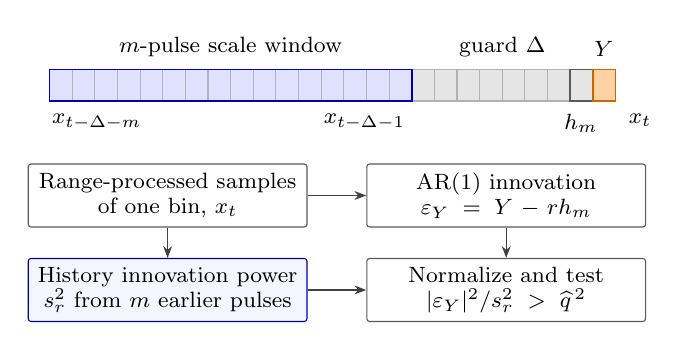
\begin{tikzpicture}[x=1mm,y=1mm,font=\fontsize{8}{9}\selectfont,
  box/.style={draw=black!65,rounded corners=1pt,align=center,
    inner sep=2pt,text width=34mm,minimum height=8mm,fill=white},
  arr/.style={-{Stealth[length=1.5mm]},draw=black!75,line width=0.5pt}]
% The timeline shows one bin; h_m remains the latest predictor sample.
\fill[blue!12] (5,18) rectangle (51,22);
\fill[black!10] (51,18) rectangle (74,22);
\fill[orange!35] (74,18) rectangle (76.875,22);
\foreach \i in {0,...,24} {
  \pgfmathsetmacro{\cellx}{5+2.875*\i}
  \draw[black!30] (\cellx,18) rectangle ++(2.875,4);
}
\draw[blue!70!black,line width=0.6pt] (5,18) rectangle (51,22);
\draw[black!65,line width=0.6pt] (71.125,18) rectangle (74,22);
\draw[orange!80!black,line width=0.6pt] (74,18) rectangle (76.875,22);
\node[anchor=south] at (28,22.4) {$m$-pulse scale window};
\node[anchor=south] at (62.5,22.4) {guard $\Delta$};
\node[anchor=south] at (75.4,22.4) {$Y$};
\node[anchor=north] at (11,17.6) {$x_{t-\Delta-m}$};
\node[anchor=north] at (45,17.6) {$x_{t-\Delta-1}$};
\node[anchor=north] at (72.5,17.6) {$h_m$};
\node[anchor=north] at (80,17.6) {$x_t$};
% Two branches supply the numerator and its history scale.
\node[box] (a) at (20,6) {Range-processed samples\\of one bin, $x_t$};
\node[box] (w) at (63,6) {AR(1) innovation\\$\varepsilon_Y=Y-rh_m$};
\node[box,draw=blue!70!black,fill=blue!4] (s) at (20,-6) {History innovation power\\$s_r^2$ from $m$ earlier pulses};
\node[box] (q) at (63,-6) {Normalize and test\\$|\varepsilon_Y|^2/s_r^2>\widehat q^{\,2}$};
\draw[arr] (a.east)--(w.west);
\draw[arr] (a.south)--(s.north);
\draw[arr] (w.south)--(q.north);
\draw[arr] (s.east)--(q.west);
\end{tikzpicture}
\caption{Cell-wise detection after range processing. The scale uses $x_{t-\Delta-m},\ldots,x_{t-\Delta-1}$; the predictor retains the latest sample $h_m=x_{t-1}$, including when it lies in the guard. The AR coefficient is fitted on clutter training data and $\widehat q$ on clean calibration episodes. The diagram shows the squared score and threshold.}
\label{fig:chain}
\end{figure}

\subsection{Conformal thresholds}
For a score $T$ and a design false-alarm rate $\alpha$, the threshold $\widehat q$ is the $k_\alpha$-th smallest value of $T$ over $n$ clean calibration episodes, with $k_\alpha=\lceil(n+1)(1-\alpha)\rceil$ and $\widehat q=+\infty$ if $k_\alpha=n+1$. For exchangeable calibration and test episodes, the false-alarm probability is then at most $\alpha$ \cite{lei2018,bates2023}. Section~\ref{sec:calib} gives its distribution given the calibration set.

\section{Laws of Whitened-Innovation Detection}\label{sec:laws}
The laws follow a target through the detector, from the tested pulse at onset to a target that persists into the history and a dwell of several pulses; the calibration and certification of the threshold close the section.

\subsection{The exact law at onset}\label{sec:onsetlaws}
\begin{proposition}\label{prop:law}
For $q>0$, let $X\sim\mathcal{CN}(0,\Sigma)$, $\Sigma\succ0$, fix a linear center $a^{\mathsf T}H$ and a scale $s(H)^2=H^{\mathsf H}QH/m$ with $Q\succeq0$, $Q\ne0$, and let $\lambda_k$ be the nonzero eigenvalues, with multiplicity, of $\Sigma^{1/2}M_q\Sigma^{1/2}$, $M_q=\bar bb^{\mathsf T}-\frac{q^2}{m}\operatorname{diag}(Q,0)$, $b=e_{m+1}-(a^{\mathsf T},0)^{\mathsf T}$. Exactly one eigenvalue $\lambda_+$ is positive, and
\begin{equation}
G_\Sigma(q):=\PP\{|Y-a^{\mathsf T}H|\le q\,s(H)\}=1-\prod_{k\ne+}\frac{\lambda_+}{\lambda_+-\lambda_k}.
\label{eq:exactlaw}
\end{equation}
\end{proposition}
The proof (Appendix~\ref{app:law}) holds for any multiplicities. Equation \eqref{eq:exactlaw} specializes classical real and complex Gaussian quadratic-form theory \cite{imhof1961,alnaffouri2016}. At the true AR(1) coefficient it is the CA law $1-(1+q^2/m)^{-m}$ \cite{finn1968,gandhi1988} applied to innovations. It evaluates coverage, the probability that the next sample falls inside the prediction disc, at any linear center and quadratic scale, texture and noise level, without simulation.
\begin{corollary}\label{cor:texture}
With $\nu=0$, \eqref{eq:exactlaw} does not depend on the texture. With $\nu>0$ texture invariance is generally lost \cite{gini1997,watts1987}; the CNR-conditional coverage is $c\mapsto G_{cR+I}(\widehat q)$, which tends to the pure-clutter value as $c\to\infty$ and to $G_I(\widehat q)$ as $c\to0$.
\end{corollary}
\begin{corollary}\label{cor:detect}
A Swerling-1 target $\sqrt{SP}\,g\,v$ ($P$ the local clutter-plus-noise power, $S$ the SCR relative to it, $g\sim\mathcal{CN}(0,1)$, $v$ the target signature over the episode) is detected with $P_{\rm d}=1-G_{\Sigma+SP\,vv^{\mathsf H}}(\widehat q)$. For a target in $Y$ only, pure AR(1) clutter and the true coefficient,
\begin{equation}
P_{\rm d}=\Big(1+\frac{q^2}{m}\,\frac{1-|\rho|^2}{1-|\rho|^2+S}\Big)^{-m},
\label{eq:pdclosed}
\end{equation}
the CA-CFAR law with the SCR multiplied by the whitening factor $1/(1-|\rho|^2)$.
\end{corollary}
Because the clutter innovation powers are conditionally independent exponentials, the OS-CFAR law also holds at onset.
\begin{corollary}\label{cor:os}
With $\nu=0$, AR(1) speckle and $r=\rho$, the OS score with the $k$-th smallest of $m$ innovation powers has $\PP\{\text{exceedance}\}=\prod_{i=0}^{k-1}(m-i)/(m-i+q^2)$ for every texture, the OS-CFAR law \cite{rohling1983}; a target in $Y$ only is detected with this probability, $q^2$ replaced by $q^2/\{1+S/(1-|\rho|^2)\}$.
\end{corollary}

\subsection{Thermal noise caps the whitening gain}
\begin{proposition}\label{prop:gain}
Under \eqref{eq:r7model} with AR(1) speckle, testing the prediction error against its own variance gains, over power-only detection and for a long history, $G_{\rm IN}(c)=(1+c)/\{c(1+|r|^2-2\Re\bar r\rho)+1+|r|^2\}$ for the IN-ARCP center and $G_{\rm opt}(c)=(1+c)/V(c)\ge\max\{1,G_{\rm IN}\}$ for the optimal predictor, with $V=\frac12(\xi+\sqrt{\xi^2-4|\rho|^2})$ and $\xi=1+|\rho|^2+c(1-|\rho|^2)$.
\end{proposition}
The prediction error $Y-rH_m$ is a weighted two-pulse canceller, and $G_{\rm IN}$ is its clutter attenuation, which equals its improvement factor for a target in $Y$ alone \cite{richards2014}. In noise-dominated cells, first-order normalization loses up to $10\log_{10}(1+|\rho|^2)$~dB, which the NA score avoids (proof in the Supplementary Material).

\begin{figure*}[!t]
\centering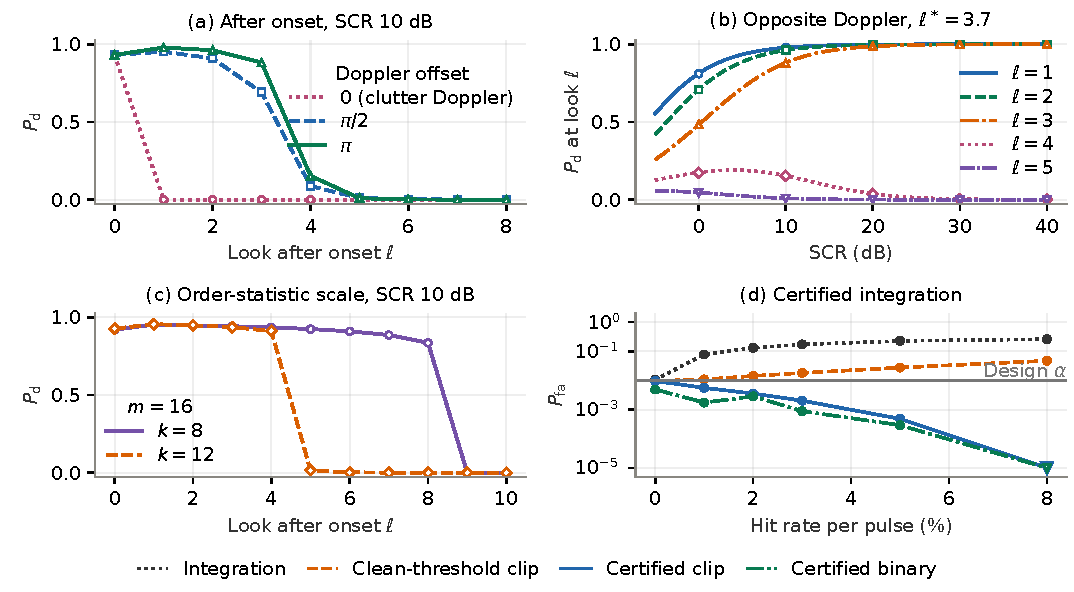
\includegraphics[width=\textwidth]{fig_theory_row.pdf}
\caption{Closed forms (lines) against Monte Carlo (markers; $10^5$ episodes per point, $5\times10^4$ in (b)) at the true coefficient, AR(1) compound-Gaussian clutter with $\rho=0.93e^{-0.2\mathrm j}$, lognormal texture, $m=16$, $P_{\rm fa}=0.01$. (a) Proposition~\ref{prop:rank1}; (b) horizon, Corollary~\ref{cor:horizon}; (c) OS scales (quadrature); (d) Theorem~\ref{thm:cert}, $P_{\rm fa}$ against the hit rate for Gaussian interference 30~dB above the local power, Monte Carlo only (open downward triangles: no event in $10^5$).}
\label{fig:theory}
\end{figure*}
\subsection{Persistent targets}
A target that remains in the beam after its onset enters the history that normalizes it; in the limit of a strong target present in every sample, the score cannot detect it.
\begin{proposition}\label{prop:blind}
For $m>1$, $|r|<1$ and a persistent target $A(e^{\mathrm j\omega t})_{t=1}^{m+1}$ in every sample, the IN-ARCP score tends as $|A|\to\infty$ to
\[
\begin{aligned}
T_\infty&=\frac{\sqrt m\,|1-re^{-\mathrm j\omega}|}
{\sqrt{(1-|r|^2)+(m-1)|1-re^{-\mathrm j\omega}|^2}}\\
&\le\sqrt{\frac{m}{m-1}}.
\end{aligned}
\]
Thus $P_{\rm d}\to0$ whenever $\widehat q>\sqrt{m/(m-1)}$.
\end{proposition}
To follow a target that starts at a known pulse, we fix the model for the rest of this section: the speckle is AR(1) with coefficient $\rho$, $\nu=0$ and $r=\rho$ (Theorem~\ref{thm:cert} needs none of these assumptions). The innovations $\varepsilon_1=\sqrt{1-|\rho|^2}\,x_1$ and $\varepsilon_t=x_t-\rho x_{t-1}$ are then independent $\mathcal{CN}(0,\sigma_e^2)$ given the texture, and every statistic below is homogeneous of degree zero, so the texture cancels. A Swerling-1 target $\sqrt{SP}\,g\,e^{\mathrm j\omega t}$, $g\sim\mathcal{CN}(0,1)$ common to all pulses, that starts at pulse $t_0$ contributes $g\sqrt{S_w}$ to $\varepsilon_{t_0}$ and $g\sqrt{S_w}\,d(\omega)e^{\mathrm j\omega t}$ to $\varepsilon_t$, $t>t_0$, where
\begin{equation}
\begin{gathered}
S_w=\frac{S}{1-|\rho|^2},\qquad |d(\omega)|^2=|1-\rho e^{-\mathrm j\omega}|^2,\\
S_w|d(\omega)|^2=S\,w(\omega),\qquad w(\omega)=\frac{P}{S_c(\omega)},
\end{gathered}
\label{eq:whitenedscr}
\end{equation}
and $S_c(\omega)=P(1-|\rho|^2)/|1-\rho e^{-\mathrm j\omega}|^2$ is the clutter spectrum. Under $H_0$, whitening yields conditionally independent exponential innovation powers. It multiplies the SCR by $1/(1-|\rho|^2)$ in the onset pulse and by $w(\omega)$ after it; for AR($p$) speckle, $d(\omega)$ is the whitening filter's response. Self-masking is classical for clutter maps \cite{lops1989,naldi1999}; to our knowledge, the post-onset law with its horizon, the OS law under persistence and the certificate are new in this form.

\subsection{After the onset: a rank-one law and a visibility horizon}
\begin{proposition}\label{prop:rank1}
Let the innovation-normalized score with $m$ history innovations be thresholded at $q>0$, and let a Swerling-1 target have whitened energy $\mathcal E_0$ in the tested innovation and $\mathcal E_H$ in the history innovations. With $\beta=q^2/m$, let $\lambda_\pm$ be the roots of
\[
\lambda^2-(1+\mathcal E_0-\beta-\beta\mathcal E_H)\lambda-\beta(1+\mathcal E_0+\mathcal E_H)=0 .
\]
Then $\lambda_+>0>\lambda_-$ and
\begin{equation}
P_{\rm d}=\frac{\lambda_+}{\lambda_+-\lambda_-}\Big(1+\frac{\beta}{\lambda_+}\Big)^{-(m-1)}.
\label{eq:rank1}
\end{equation}
For a persistent target observed at look $1\le\ell\le m-1$, $\mathcal E_0=S_w|d(\omega)|^2$ and $\mathcal E_H=S_w\{1+(\ell-1)|d(\omega)|^2\}$; at onset ($\ell=0$), $\mathcal E_0=S_w$, $\mathcal E_H=0$, and \eqref{eq:rank1} reduces to \eqref{eq:pdclosed}.
\end{proposition}
\begin{corollary}\label{cor:horizon}
For $1\le\ell\le m-1$, as $S\to\infty$ the look-$\ell$ detection probability tends to one if $\ell<\ell^*$ and to zero if $\ell>\ell^*$, where
\begin{equation}
\ell^*(\omega)=1+\frac{m}{q^2}-\frac{1}{|d(\omega)|^2}.
\label{eq:horizon}
\end{equation}
\end{corollary}
Since $\ell^*<1+m/q^2$, a strong target is kept for fewer than $1+m/q^2$ post-onset looks, and not near clutter Doppler, where $|d(\omega)|^2\approx(1-|\rho|)^2$. At $m=16$ and $P_{\rm fa}=0.01$, $m/q^2=3.0$; for $|\rho|=0.93$ the horizon is \ThHorizonOpp{} looks at opposite Doppler and negative at clutter Doppler (Fig.~\ref{fig:theory}a,b). A guard delays scale contamination. Keep the tested energy $\mathcal E_0$ unchanged; set $\mathcal E_H=0$ for $\ell\le\Delta$ and use the history energy at $\ell-\Delta$ thereafter. Beyond the guard, the critical value is $\Delta+\ell^*$; the false-alarm law is unchanged.

With the OS scale, the target occupies $\ell$ history innovations after the onset, and $P_{\rm d}$ is a two-dimensional integral (quadrature). For a strong target and $\ell\le m-k$, the contaminated powers lie above the scale, which becomes the $k$-th smallest of $m-\ell$ clean powers, and
\begin{equation}
P_{\rm d}\simeq\prod_{i=0}^{k-1}\frac{m-\ell-i}{m-\ell-i+q^2/(1+S_w|d|^2)},\qquad \ell\le m-k,
\label{eq:osstrong}
\end{equation}
while $P_{\rm d}\to0$ for $\ell>m-k$ provided $q^2>\max\{1,|d(\omega)|^2\}$, as in the settings tested (Fig.~\ref{fig:theory}c).

\subsection{Dwell integration and self-normalized Doppler}
Over a dwell, non-coherent integration of $K$ innovation powers against the mean of $m$ history powers, at threshold $\theta$ and with $\tau=\theta/m$, has
\begin{equation}
P_{\rm fa}=\sum_{i=0}^{K-1}\binom{m+i-1}{i}\frac{\tau^i}{(1+\tau)^{m+i}},
\label{eq:dwellpfa}
\end{equation}
and a Swerling-1 target starting at the first dwell pulse, with clean history, whitened energy $\mathcal E_D=S_w\{1+(K-1)|d|^2\}$, $\delta=1+\mathcal E_D$ and $\tau'=\tau(1-1/\delta)$, has
\begin{multline}
P_{\rm d}=\sum_{i=0}^{K-2}\binom{m+i-1}{i}\frac{\tau^i}{(1+\tau)^{m+i}}+\Big(1-\frac1\delta\Big)^{-(K-1)}\\
\times\Big[\Big(1+\frac{\tau}{\delta}\Big)^{-m}-\sum_{i=0}^{K-2}\binom{m+i-1}{i}\frac{\tau'^{\,i}}{(1+\tau)^{m+i}}\Big],
\label{eq:dwellpd}
\end{multline}
the CA non-coherent-integration law \cite{gandhi1988,richards2014} with the whitened energy. For clutter power summed over $K$ correlated pulses, matching the conditional mean and variance gives $K_{\rm eff}=K^2/\sum_{i,j}|\rho|^{2|i-j|}$ effective looks (\ThKeff{} for $K=8$ at $|\rho|=0.93$).

The P-ANMF divides the periodogram of $N$ whitened innovations by their energy. For a known on-grid Doppler and a target present before the dwell, the statistic is Beta$(1,N-1)$ under $H_0$ for every texture, and
\begin{equation}
P_{\rm d}=\Big[1+\frac{P_{\rm fa}^{-1/(N-1)}-1}{1+N S\,w(\omega)}\Big]^{-(N-1)},
\label{eq:panmf}
\end{equation}
the normalized-matched-filter law \cite{kraut1999,conte1995} with the whitened SCR. Maximizing over the $N$ DFT bins gives Fisher's $g$ statistic \cite{fisher1929g}; inclusion--exclusion gives its null law and, with one ordinate of increased mean, its Swerling-1 detection law (Supplementary Material). Dwell normalization avoids the history self-masking of Proposition~\ref{prop:blind}.

\subsection{Conformal calibration}\label{sec:calib}
For i.i.d.\ continuous scores and $k_\alpha\le n$, the false-alarm probability given the $n$ calibration scores is Beta$(n+1-k_\alpha,k_\alpha)$ \cite{vovk2012}. With ties, as for clipped or binary statistics, $\PP\{T>\widehat q\}\le\alpha$ still holds, conservatively. Because $k_\alpha$ is a ceiling, $\PP\{P_{\rm fa}>2\alpha\}$ is not monotone in $n$. It first falls below 0.05 at $n=149$, 1,497 and 14,978 for $\alpha=10^{-2},10^{-3},10^{-4}$, and it stays below for every $n$ beyond about $3.15/\alpha$. Our $10^{-4}$ calibration sets of \LowCalMin--\LowCalMax{} per-look episodes and \DwellCalMin--\DwellCalMax{} dwell segments give \LowCalPtwoMin--\LowCalPtwoMax. These Beta calculations require independence; non-overlap alone does not validate them for correlated radar episodes. For a known-scale Swerling-1 detector, the expected $P_{\rm d}$ under calibration is a ratio of Beta functions, from which the CFAR loss of a conformal threshold follows \cite{watts2007cfarloss} (Supplementary Material).

\subsection{Certified integration under pulsed interference}\label{sec:certsec}
Pulsed interference (asynchronous pulses of another radar, jamming pulses or FMCW chirp crossings) corrupts a few pulses with interference of arbitrary, unknown power. We call such a corrupted pulse a \emph{hit}, to distinguish it from an exceedance, a statistic above its threshold. For the whitened statistics, a hit at pulse $t_{\rm h}$ corrupts the innovations $t_{\rm h},\dots,t_{\rm h}+p$. The clipped integrator $T=\sum_{i=1}^K\min\{|\varepsilon_{m+i}|^2/s_{k_H}^2,\kappa\}$ and its binary counterpart admit a certificate that does not depend on the interference power.
\begin{theorem}\label{thm:cert}
For a clean episode $x$ and a set $\mathcal J$ of corrupted innovations, let $W(x,\mathcal J)$ be $T$ computed with the corrupted history powers set to zero and the corrupted dwell terms set to $\kappa$ (binary: counted as exceedances). If this scale is zero, set $W=K\kappa$ (binary: $K$). Then $T\le W(x,\mathcal J)$ for every interference value, and $W$ is nondecreasing in $\mathcal J$. Let $\widehat q$ be the split-conformal quantile of $W(X_i,\mathcal J_i)$ over clean calibration episodes $X_i$, with masks drawn i.i.d.\ from $\mathcal D$, independently of all clean episodes and of the test hit set. If those episodes are exchangeable and the test hit set is independent of all clean episodes and dominated by $\mathcal D$ in the inclusion order (a coupling $\mathcal J\subseteq\tilde{\mathcal J}\sim\mathcal D$ exists), the false-alarm probability is at most $\alpha$ for any interference amplitudes, including adversarial ones.
\end{theorem}
A bound on the hit rate alone does not give this dominance: periodic or bursty interference with the same rate can put more hits into one segment than independent hits do. A trimmed sum, which discards the largest dwell terms, uses the same bound with corrupted dwell terms set to $+\infty$. Its population threshold is infinite if the probability of more corrupted terms than discarded exceeds $\alpha$; finite-sample thresholds also depend on the sampled masks. We discard the fewest terms for which this probability is at most $\alpha/5$: \TrimTwo{} of eight at a 2\% hit rate and $\alpha=10^{-2}$, since a hit corrupts two AR(1) innovations. Fig.~\ref{fig:theory}d checks the theorem in simulation.


\section{Experimental Design}\label{sec:design}
\emph{IPIX sea clutter.} The 14 openly available Dartmouth 1993 stare sessions of the McMaster IPIX radar \cite{ipixweb}: X-band, 1~kHz pulse repetition, 14 range cells of 15~m, six dates with wave heights of 0.8--3.8~m \cite{haykin1995}. Preprocessing follows the providers' recipe. Target cells and one guard cell on each side are excluded from clutter; Section~\ref{sec:realtarget} uses the primary target cell. The two like-polarized channels are analyzed separately. Each session is split into thirds, separated by 2,000-pulse gaps, that serve as training, calibration and test data. One of the three assignments of these roles was used while the methods were developed; the other two give the \NUnitsConf{} evaluation units (session $\times$ channel $\times$ assignment), which therefore reuse recordings seen during development and are not an untouched confirmation. Day transfer and two series held out until the end are in the Supplementary Material.

\emph{77~GHz FMCW data.} The open JKU parking-lot dataset \cite{jku2026}: 76--77~GHz chirp sequences (34~$\mu$s chirp period, 128 chirps per frame, 100 frames) recorded by two radar stations observing a static scene of parked cars, with a clean reference run and runs with an unsynchronized interferer, dense (scenario A, \JHitA\% of chirps hit) and sparse (scenario C, \JHitC\%). A further scenario-A run adds a walking person. A chirp counts as a hit when more than 10\% of its range bins exceed ten times the reference run's median power.

\emph{NetRAD S-band sea clutter.} Fourteen recordings of the open NetRAD data \cite{netrad2026,fioranelli2016netrad}: 2.4~GHz, 45~MHz chirp, 1~kHz pulse repetition, monostatic node, Cape Peninsula, 9 June 2011, seven HH and seven VV recordings of 130~s, with the providers' clutter range cells (41--101 per recording). No statistic was computed on these data before their protocol was frozen. Detectors and settings are those used on IPIX, except that the ANMF secondary data come from the cells two to four cells away (15--30 vectors). The 28 units are recording $\times$ assignment, and intervals resample recordings. A pulse is flagged when more than 10\% of its range bins exceed ten times the bin's median power over the recording. Whether flagged pulses are interference or range-extended sea spikes is not established.

\emph{Protocols.} Each study's methods, settings, metrics and expected outcomes were recorded in a hashed protocol before computing outcomes (an internal record, not an external registry). Subsequent analyses are labeled exploratory. Of the 53 predicted outcomes for four final studies, 13 were not met and 4 pedestrian outcomes (Section~\ref{sec:detect}) received no verdict. The Supplementary Material lists both and all protocol deviations.

\emph{Detectors and thresholds.} Per-look scores use $m=16$. Dwell detectors use a 16-pulse history and an 8-pulse dwell that starts at the first full-amplitude target pulse (the same idealization for every detector), the median as OS history scale, clip level $\kappa=6$ (4 to 18 in a clip-level comparison) and binary threshold $\eta=6$. The ANMF uses secondary vectors from clutter cells at least two cells away, at five time positions (20--35 vectors). Power detectors normalize by the same 16 history samples (CA16) or by the cell's power over $\pm1024$ pulses (CAloc, non-causal). Conformal thresholds are calibrated on clean episodes from the calibration third. For the low-false-alarm analysis these episodes do not overlap (\LowCalMin--\LowCalMax{} per unit; \DwellCalMin--\DwellCalMax{} dwell segments). Model-based thresholds are the laws of Section~\ref{sec:laws} at the fitted model, Gaussian plug-ins, the Kraut--Scharf and fixed-point ANMF laws, Gaussian simulation and an AR residual bootstrap of the sieve type \cite{qu2024sieve}.

\emph{Targets, interference and statistics.} Swerling-1 targets are injected from $-5$ to 25~dB SCR relative to local power: at onset, persistent from a given pulse with random Doppler, or rising linearly over $L$ pulses. Both IPIX test segments and secondary data receive independent pulse hits with probability $p_{\rm h}\in\{0.02,0.05\}$ and complex Gaussian amplitude 10 or 30~dB above local power. On the 77~GHz data, injected beat-tone targets pass through the same raw-sample processing. The 95\% intervals use six-day cluster bootstrap resampling (10,000 replicates). They are approximate with six clusters; leave-one-day-out ranges are in the Supplementary Material.

\begin{table}[!t]
\centering\footnotesize
\caption{Measured false-alarm rate / design $\alpha$ on IPIX test thirds (\NUnitsConf{} units, pooled). Conformal: split-conformal threshold. Model-based: the rule in parentheses at the fitted model. Bold: outside $[0.5,2]$. Day-cluster intervals are in Supplementary Table~S2; at $10^{-4}$ each unit contributes \FaPerUnitMin--\FaPerUnitMax{} expected false alarms.}
\label{tab:lowpfa}
\setlength{\tabcolsep}{2.0pt}
\begin{tabular}{lcccccc}
\toprule
 & \multicolumn{3}{c}{Conformal} & \multicolumn{3}{c}{Model-based rule}\\
\cmidrule(lr){2-4}\cmidrule(lr){5-7}
$\alpha$ & $10^{-2}$ & $10^{-3}$ & $10^{-4}$ & $10^{-2}$ & $10^{-3}$ & $10^{-4}$\\
\midrule
\emph{Per look} &&&&&&\\
IN-ARCP (CA law) & 1.01 & 1.03 & 0.73 & 0.96 & 1.02 & 1.92\\
\quad residual bootstrap &  &  &  & 1.63 & \textbf{2.43} & \textbf{4.27}\\
IN-AR(4) (CA law) & 1.00 & 1.02 & 0.86 & 1.03 & 1.19 & \textbf{2.73}\\
OS scale, $k=8$ (OS law) & 1.04 & 1.02 & 0.92 & \textbf{2.15} & \textbf{8.34} & \textbf{45.9}\\
NA-AR(4) (Gaussian) & 1.00 & 1.05 & 1.04 & 1.56 & \textbf{2.79} & \textbf{7.46}\\
Power, CA (white law) & 1.00 & 1.00 & 0.75 & 0.80 & 0.56 & \textbf{0.49}\\
Power, OS (white law) & 1.01 & 0.98 & 0.75 & \textbf{2.07} & \textbf{5.56} & \textbf{18.3}\\
\emph{Eight-pulse dwell} &&&&&&\\
Integration (law \eqref{eq:dwellpfa}) & 1.02 & 1.05 & 1.02 & \textbf{2.02} & \textbf{4.35} & \textbf{14.3}\\
PAMF-H, one Doppler (CA law) & 0.99 & 1.00 & 0.89 & 1.97 & \textbf{3.66} & \textbf{9.88}\\
P-ANMF, one bin (Beta) & 1.10 & 1.14 & 1.10 & 1.78 & \textbf{3.05} & \textbf{5.47}\\
P-ANMF, max (Fisher's $g$) & 1.04 & 1.04 & 1.47 & \textbf{4.36} & \textbf{13.1} & \textbf{49.6}\\
ANMF-SCM (Kraut--Scharf) & 1.06 & 1.04 & 0.85 & \textbf{2.02} & \textbf{3.57} & \textbf{8.07}\\
ANMF-Tyler (FP law) & 1.04 & 1.05 & 0.82 & 1.62 & \textbf{2.66} & \textbf{6.01}\\
Clipped, OS scale (Gaussian sim.) & 1.05 & 0.67 & \textbf{0.03} & \textbf{4.84} & \textbf{17.2} & \textbf{59.9}\\
\bottomrule
\end{tabular}

\end{table}
\begin{figure*}[!t]
\centering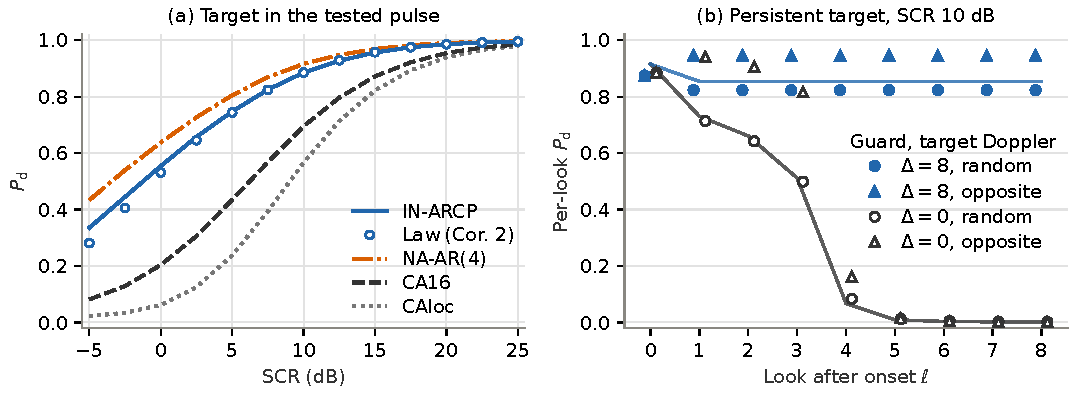
\includegraphics[width=\textwidth]{fig_detection.pdf}
\caption{Detection of Swerling-1 targets injected into IPIX test episodes ($m=16$, conformal thresholds, per-look $P_{\rm fa}=0.01$). (a) Target in the tested pulse (\DetNTest{} episodes in total). NA-AR(4): noise-aware score, \DetNAFourGainCAHalf~dB less SCR than CA16. Circles: law of Corollary~\ref{cor:detect}, model fitted on each unit's training third. Empirical and law curves are unit means; the text averages per-unit gains. (b) Persistent 10~dB target (\NUnitsConf{} units) without and with an eight-pulse guard, markers offset for visibility; means in the text are over looks 1--8. Markers: episode-weighted means; lines: unit-mean law of Proposition~\ref{prop:rank1} at fitted AR(1) coefficients, random Doppler (exploratory).}
\label{fig:detect}
\end{figure*}
\section{Results}\label{sec:results}
\subsection{False-alarm control across clutter power and down to \texorpdfstring{$10^{-4}$}{1e-4}}\label{sec:fa}
Table~\ref{tab:lowpfa} is the central calibration result. Conformal thresholds keep the measured rate of twelve of the thirteen statistics within \LConfMinThree--\LConfMaxThree{} times design at $10^{-3}$ and \LConfMinFour--\LConfMaxFour{} times at $10^{-4}$ (IN-ARCP: \InConfFour{} [\InConfFourLo, \InConfFourHi]). The exception is the clipped integrator, which is conservative (\LClipConfThree{} and \LClipConfFour) because its statistic saturates at $K\kappa$ and ties at the threshold. At $10^{-2}$ some ratios lie slightly above one, such as \PanmfBinConfTwo{} [\PanmfBinConfTwoLo, \PanmfBinConfTwoHi] for the one-bin P-ANMF. These exceed sampling noise and suggest that the calibration and test thirds of a session are not exactly exchangeable, as the non-stationarity of sea clutter implies \cite{greco2010}. Bounding the coverage gap that leaves would need a budget for the drift between the thirds \cite{barber2023}.

Model-based thresholds, by contrast, fail in the tail. At $10^{-4}$, \NWhitenedLawsFail{} of the \NWhitenedLaws{} model-based laws of the whitened statistics and the ANMF exceed twice the design rate, by up to \LAnalMaxFour-fold (bold entries in Table~\ref{tab:lowpfa}). The ANMF laws fail already at $10^{-3}$, at \LScmThree{} (SCM) and \LFpThree{} (Tyler) times design. The Kraut--Scharf law fails 2.8--3.4-fold at $10^{-2}$ even in simulated compound-Gaussian clutter (Supplementary Material). The SCM failure is therefore already present under the model, and need not come from any departure of real clutter from it. A residual bootstrap of real innovations still exceeds design \LBootFour-fold at $10^{-4}$, consistent with dependence among an episode's innovations, which independent resampling discards. The laws fail in at least two ways (exploratory). The rate of the OS and Fisher's-$g$ laws depends strongly on clutter power: texture-quintile spread \AnalSpreadOsThree{} and \AnalSpreadFisherThree{} at $10^{-3}$, against \AnalSpreadInThree{} for the CA law. The clipped and ANMF rules fail almost evenly across it (\AnalSpreadClipThree--\AnalSpreadFpThree). The only law that stays within twofold is the CA law of the IN-ARCP score (\LInAnalThree{} at $10^{-3}$; \LInAnalFour{} [\InAnalFourLo, \InAnalFourHi] at $10^{-4}$, still above design), plausibly because its scale averages all 16 history innovations.

The false-alarm rate should also stay constant across clutter power. At a design of 0.01, the conformal false-alarm rate of IN-ARCP ranges from \QPfaINMin{} to \QPfaINMax{} over texture quintiles, a max/min spread of \QPfaINSpread{} (\LInConfSpreadFour{} at $10^{-4}$ in the low-false-alarm analysis). Without normalization the spread is \QPfaUSpread; normalization by the raw history RMS gives \QPfaRMSSpread. Normalizing by the raw history RMS therefore does not keep the score pivotal---its null free of the clutter power---whereas innovation normalization approximately does where clutter dominates noise. In the larger low-false-alarm calibration sets it is \NetSpreadInIpix{} for IN-ARCP and \NetSpreadCaIpix{} for CA16, which is thus more pivotal still but needs \DetINGainCAHalf~dB more SCR.

On the 77~GHz data, thermal noise breaks the texture invariance as Corollary~\ref{cor:texture} predicts. From the lowest CNR class to the 10--20~dB class, IN-ARCP coverage at a design of 0.90 rises from \JInLow{} to \JInHigh{}, more than the law's \JPredHigh{} (mean absolute deviation over all classes \JMae), and the false-alarm rate at $10^{-2}$ falls further than predicted (post hoc; Table~\ref{tab:map}).

\subsection{Detection of new returns}\label{sec:detect}
Fig.~\ref{fig:detect}a shows targets that appear in the tested pulse. At $P_{\rm d}=0.5$, IN-ARCP needs \DetINGainCAHalf~dB [\DetINGainCALoHalf, \DetINGainCAHiHalf] less SCR than power detection on the same pulses (CA16) and \DetINGainLocHalf~dB less than the long-window power detector (CAloc; \DayGainMin--\DayGainMax~dB by day, post hoc). The exact law of Corollary~\ref{cor:detect} predicts $P_{\rm d}$ with a mean absolute error of \DetMae{} per unit and SCR. It attributes the shortfall from the clutter-only whitening factor (\DetNaiveGain~dB) to thermal noise (Proposition~\ref{prop:gain}). At this design rate the Gaussian threshold of IN-ARCP gives the same sensitivity at a similar false-alarm rate, so the gain comes from whitening, not from calibration.

Over an eight-pulse dwell (SCR table in the Supplementary Material), PAMF-H is the most sensitive detector, and AR non-coherent integration is close to it. The ANMF (Tyler) needs at least \AFpMinusPamf~dB [\AFpMinusPamfLo, \AFpMinusPamfHi] more SCR than PAMF-H; this is a lower bound, because PAMF-H reaches $P_{\rm d}=0.5$ at the lowest SCR tested. The P-ANMF pays for normalizing by a dwell that contains the target. The clipped integrator costs \AClipMinusDin~dB [\AClipMinusDinLo, \AClipMinusDinHi] against AR(1) integration at $\alpha=0.01$, and the binary integrator costs more. The power OS detector on the cell's own history (clutter-map OS-CFAR) needs \AOsrawMinusIn~dB [\AOsrawMinusInLo, \AOsrawMinusInHi] more SCR than IN-ARCP at the first look, so the sensitivity comes from whitening, not from the order statistic. A Hann-windowed eight-pulse Doppler filter bank with range CA normalization needs \ClINvsMTD~dB more SCR than integrated IN-ARCP. All whitening detectors lose sensitivity for targets at the clutter Doppler (PAMF-H by \ClPAMFMatched~dB).

Real onsets come from the 77~GHz pedestrian run. Its dense interference is suppressed by fast-time zeroing. Then one chirp per frame (200~ms apart) is tested against the 16 earlier frames of its bin, or its range neighbors for range CA-CFAR, at false-alarm rates of \PedPfaMin--\PedPfaMax{} times the design $10^{-2}$. Of \PedEvents{} onsets of the person's direct and bistatic returns in 15-cm range bins, marked by the radar's own range-Doppler map, IN-ARCP detects \PedIN{} within three frames (mean over 16 receiver--chirp tests), the power clutter map \PedCA, its OS form \PedOS{} and range CA-CFAR \PedRCA. Frame-to-frame clutter is nearly uncorrelated here (median $|r|=\PedR$), so Proposition~\ref{prop:gain} predicts little whitening gain, and IN-ARCP only matches the clutter map. The onsets fall in \PedBlocks{} distinct five-frame blocks, fewer than the \PedBlocksReq{} required in advance, so this result is descriptive (Supplementary Material).

\subsection{Persistent and emerging targets}\label{sec:onset}
A target that stays in the beam after its onset enters the history. As Proposition~\ref{prop:rank1} predicts, IN-ARCP then loses it (Fig.~\ref{fig:detect}b): at 10~dB its per-look $P_{\rm d}$ falls from \OnLookZero{} at onset to \OnLookFour{} at look 4. A target at the clutter Doppler is already lost at look 1 (\OnMatchedOne), whereas one at the opposite Doppler is still detected there (\OnOppOne) and lasts several looks, in line with the visibility horizon of \ThHorizonOpp{} looks (Corollary~\ref{cor:horizon}). The exact law reproduces these decays, with mean absolute errors of \OnTheoryMaeRand, \OnTheoryMaeMatch{} and \OnTheoryMaeOpp{} for random, clutter and opposite Doppler (exploratory).

A guard of eight pulses keeps the target out of the scale. With it, the per-look $P_{\rm d}$ over the eight guarded looks averages \GuardMeanLookEight{} for random and \GuardOppEight{} for opposite Doppler, against \GuardMeanLookZero{} without the guard for random Doppler. The law gives \GuardLawEight{} (exploratory), and the conformal false-alarm rate stays at \GuardPfaEight{} times design. No look beyond the \GuardLooksMeasuredOrd{} was measured on these data; Monte Carlo confirms the same decay delayed by $\Delta$ (Supplementary Material). The guard costs \GuardOnsetCost~dB at onset, more than the protocol allowed for, and a 16-pulse guard \GuardOnsetCostSixteen~dB for the same \GuardMeanLookSixteen{} over the looks measured. Those looks cannot separate the two, and the horizon $\Delta+\ell^*$ puts the longer guard's eight looks further out. At 10~dB it offers little help at clutter Doppler, where whitening strongly attenuates the target (\GuardMatchedEight). The median OS score also keeps the target ($P_{\rm d}$ \OsPersFirst--\OsPersLast), but it costs \OsCostEight~dB for abrupt targets, above the \OSLossEight~dB predicted by Corollary~\ref{cor:os}; the guard is cheaper.

Targets that emerge gradually are harder for the per-look screen. When the target amplitude rises linearly over $L$ pulses, reaching full amplitude at the first look, IN-ARCP's first-look gain over CAloc falls from \RampGainOne~dB for an abrupt onset in the ramp comparison to \RampGainEight~dB for $L=8$. At $L=16$ the target is barely detected ($P_{\rm d}=\RampPdSixteen$ at 10~dB), whereas PAMF-H over the dwell loses only \RampPAMFLoss~dB. The exact law reproduces the ramps (mean absolute error \RampMae). The ramp fills the normalizing history, and with the eight-pulse guard the probability of detecting a 16-pulse ramp within eight looks at 10~dB rises from \GuardRampZero{} to \GuardRampEight.

\label{sec:realtarget}The IPIX reference target tests the opposite extreme. It is present throughout each recording, so it lies in every history and no guard helps. Proposition~\ref{prop:blind} explains it, and a pre-specified test measures it for IN-ARCP and the clipped integrator: both exceed on the target cell at \TargetBlindRate{} at $\alpha=10^{-3}$, below their clutter rates. Self-normalized whitened Doppler detects the target with $P_{\rm d}=\TPanmfEight$ over 8 pulses and \TPanmfTwoFiveSix{} over 256 pulses. Its measured clutter false-alarm rates are \TPanmfPfaEight{} and \TPanmfPfaTwoFiveSix{} times the design $10^{-3}$. Its rate is also strongly texture-dependent (exploratory): the quintile spread is \ConfSpreadPanmfTwo{} at $10^{-2}$ and \ConfSpreadPanmfFour{} at $10^{-4}$, against \ConfSpreadInTwo{} and \LInConfSpreadFour{} for IN-ARCP, consistent with the loss of texture invariance under additive noise (Corollary~\ref{cor:texture}); the cause was not isolated. Range CA integration barely detects the target ($P_{\rm d}\le\TCaMax$), and the ANMF reaches \TFpEight--\TFpSixteen{} over 8--16 pulses. Learned detectors report $P_{\rm d}=0.91$ at $P_{\rm fa}=10^{-3}$ on IPIX with \TPanmfKiloSec-s observations and a different evaluation \cite{qu2023sensors}; over the same \TPanmfKiloPulses{} pulses the self-normalized statistic reaches \TPanmfThousand{} at $\TPanmfPfaThousand\times10^{-3}$ (pre-specified, descriptive). The target-trained classifier and the clutter-calibrated statistic use different evaluation protocols, so these rates are descriptive. Our measured false-alarm rate exceeds $2\alpha$; no guarantee for this non-exchangeable recording follows from the i.i.d.\ Beta law.

\subsection{Pulsed interference}\label{sec:interf}
\begin{table}[!t]
\centering\footnotesize
\caption{Remedies for pulsed interference on IPIX ($\alpha=0.01$, \NUnitsConf{} units). Interference is injected 30~dB above the local power; each pulse is hit with probability $p_{\rm h}$, and bursts are eight pulses long at $p_{\rm h}=5\%$. Entries are the measured $P_{\rm fa}/\alpha$ and the $P_{\rm d}$ of a 10~dB persistent target. Trimmed: \TrimTwo{} ($2\%$) and \TrimFive{} ($5\%$) of eight terms discarded. Bold: $P_{\rm fa}/\alpha>1.2$.}
\label{tab:interf}
\setlength{\tabcolsep}{2.4pt}
\begin{tabular}{lcccccc}
\toprule
 & None & \multicolumn{2}{c}{$p_{\rm h}=2\%$} & \multicolumn{2}{c}{$p_{\rm h}=5\%$} & Bursts\\
\cmidrule(lr){2-2}\cmidrule(lr){3-4}\cmidrule(lr){5-6}\cmidrule(lr){7-7}
 Detector & $P_{\rm d}$ & $P_{\rm fa}/\alpha$ & $P_{\rm d}$ & $P_{\rm fa}/\alpha$ & $P_{\rm d}$ & $P_{\rm fa}/\alpha$\\
\midrule
Clipped, clean threshold & 0.86 & 1.10 & 0.85 & \textbf{1.28} & 0.85 & \textbf{3.98}\\
Certified clipped, $\kappa=6$ & -- & 0.55 & 0.81 & 0.12 & 0.64 & \textbf{1.25}\\
Certified clipped, $\kappa=9$ & -- & 0.53 & 0.81 & 0.14 & 0.71 & \textbf{1.66}\\
Certified trimmed & -- & 0.57 & 0.79 & 0.23 & 0.72 & \textbf{3.60}\\
Blanking, mask-matched & 0.79 & 1.08 & 0.79 & \textbf{1.21} & 0.78 & \textbf{4.14}\\
\bottomrule
\end{tabular}

\end{table}
With injected pulsed interference on IPIX at $\alpha=10^{-2}$, non-coherent integration (AR(1) or AR(4)) and PAMF-H exceed their design false-alarm probability \IPfaMinAll- to \IPfaMaxInt-fold over two hit rates and two powers, because a dwell pulse corrupted by interference is an outlier that the history does not predict. Self-normalized detectors (P-ANMF, ANMF) stay within \SelfNormIntMax{} times design but lose sensitivity.

The clip level matters at low false-alarm rates. Without interference at $10^{-3}$, $\kappa=6$ makes the clipped integrator conservative through saturation ($P_{\rm fa}/\alpha=\KappaSixPfaThree$). A pre-specified saturation rule picks $\kappa=9$ in {\KappaNineUnits} of \NUnitsConf{} units and is met by no tested level ($\kappa\le18$) in \KappaRuleUndefUnits. Applied to all units (post hoc), $\kappa=9$ gives $P_{\rm fa}/\alpha=\KappaNinePfaThree$ and raises $P_{\rm d}$ at 10~dB from \KappaSixPdThree{} to \KappaNinePdThree, with negligible loss at $10^{-2}$.

Table~\ref{tab:interf} compares the remedies with dense calibration (about \DwellSegsPerUnit{} dwell segments per unit). The certified clipped integrator stays below design, consistent with Theorem~\ref{thm:cert} under its exchangeability and hit-model assumptions. The injected hits follow the calibration hit model, so this checks the implementation and the cost, not robustness. Its $P_{\rm d}$ at 10~dB falls from \CleanClipPdTen{} with a clean threshold and no interference to \CertSixPdTwo{} at a 2\% hit rate and \CertSixPdFive{} at 5\% (\CertNinePdFive{} with $\kappa=9$). The certified trimmed sum performs similarly, and so does certified binary integration ($P_{\rm d}$ within \BinCertGapMax; exploratory, Supplementary Material). At $10^{-3}$ with 5\% hits, the certificate is vacuous for every clip level: the certified threshold detects no target.

Pulse blanking, calibrated on clean episodes blanked at hit positions from the hit model, is cheaper but not certified. It keeps $P_{\rm d}=\BlankPdFive$ at 5\% hits and stays within \BlankPfaMax{} times design at $10^{-2}$. At $10^{-3}$ with 5\% hits it exceeds design \BlankFiveThreeMin- to \BlankFiveThreeMax-fold. Eight-pulse bursts expose the hit-model boundary (Table~\ref{tab:interf}): an independent-hit certificate loses false-alarm control because dominance fails; a burst-matched certificate controls false alarms but never detects. Blanking also exceeds design.

On the 77~GHz data the interference is real and occupies whole chirps. The hit model draws random 24-chirp blocks from the hit masks of frames 0--49; the test uses frames 50--99. In the sparse run the certified clipped integrator holds the false-alarm rate at \JCertPfaC{} times design without fast-time mitigation, whereas non-coherent integration runs at \JDinPfaC{} times design overall and \JDinPfaCone{} times in segments with one or two hit chirps. Against clipping with a clean threshold, the certificate costs \JCertCostClean~dB on hit-free segments and \JCertCostAll~dB overall. In the dense run, real interference mainly masks targets rather than raising false alarms (non-coherent integration \JDinPfaA{} times design), and certification is nearly vacuous. Fast-time zeroing returns the uncertified detectors to their clean-reference false-alarm rates.

\subsection{A second sea-clutter radar}\label{sec:netrad}
\begin{table}[!t]
\centering\footnotesize
\caption{IPIX and NetRAD S-band sea clutter, same code and settings except the ANMF secondary cells (Section~\ref{sec:design}). Entries: $P_{\rm fa}/\alpha$ at $\alpha=0.01$ unless stated; guard row: per-look $P_{\rm d}$ at 10~dB, mean over looks 1--8; $P_{\rm d}$ in parentheses at 10~dB. Conformal rows: the 12 statistics other than the clipped integrator (conservative on IPIX). Injected interference 30~dB above the local power. Flagged pulses: NetRAD HH, certificate calibrated on their masks.}
\label{tab:netrad}
\setlength{\tabcolsep}{3pt}
\begin{tabular}{lcc}
\toprule
 & IPIX & NetRAD\\
\midrule
Conformal, $10^{-3}$ (12 statistics) & 0.98--1.14 & 1.01--1.36\\
Conformal, $10^{-4}$ (12 statistics) & 0.73--1.47 & 1.02--4.26\\
Model-based laws $>2\times$ at $10^{-4}$ & 10 of 11 & 9 of 11\\
IN-ARCP CA law at $10^{-4}$ & 1.92 & 1.70\\
Guard: $P_{\rm d}$ per look, $\Delta=0$ / 8 & 0.24 / 0.82 & 0.30 / 0.92\\
5\% hits: AR(1) integration & 21 & 22\\
5\% hits: certified clip ($P_{\rm d}$) & 0.12 (0.64) & 0.08 (0.92)\\
5\% bursts: blanking & 4.14 & 4.11\\
Flagged pulses: integration / certified ($P_{\rm d}$) & -- & 1.05 / 0.04 (0.04)\\
\bottomrule
\end{tabular}

\end{table}
Table~\ref{tab:netrad} repeats the key tests on NetRAD, unused in development. At 1~kHz its clutter is more correlated ($|r|=\NetAbsRMin$--\NetAbsRMax, at or near the 0.98 clamp, versus an IPIX median \IpixAbsRMed). IN-ARCP gains \NetOSGain~dB over raw-power OS at onset (Supplementary Material). The guard raises mean per-look $P_{\rm d}$ from \NetGuardZero{} to \NetGuardEight{} (law \NetLawEight, exploratory) and within-eight-look detection of a 16-pulse ramp from \NetRampZero{} to \NetRampEight.

Thresholds are refitted on NetRAD; Supplementary Table~S3 gives recording-cluster intervals. All thirteen statistics are within \NetConfMinThree--\NetConfMaxThree{} times design at $10^{-3}$. At $10^{-4}$, IN-ARCP, AR(4), OS and power scores stay within \NetPerLookMax{}, but \NetNOverTwoFourWord{} statistics exceed twice design: the noise-aware score (\NetNaFour), integration, PAMF-H and both P-ANMF statistics (up to \NetDwellMax). Exploratory attribution associates most integration and PAMF-H excess with two units whose calibration thirds lack flagged pulses (without them, \NetAttrDin{} and \NetAttrPamf). P-ANMF excess comes from one unit with flags in both thirds; fewer than half of its exceedances coincide with them. IN-ARCP's texture spread is \NetSpreadIn{} versus CA16's \NetSpreadCa{} and AR(4)'s \NetSpreadInFour{}, suggesting incomplete AR(1) whitening at the clamp.

The rule flags \NetHitHHMin--\NetHitHHMax\% of the HH pulses, in bursts of several pulses, yet uncertified non-coherent integration stays at \NetWDin{} times design at $10^{-2}$ (\NetWDinThree{} at $10^{-3}$). A certificate calibrated on these masks is nearly vacuous ($P_{\rm d}=\NetWCertPd$), plausibly because the flagged pulses are frequent and come in bursts.

\section{Discussion}\label{sec:discussion}
\subsection{Where the detector works and where it fails}\label{sec:limits}
% Read-only review proposal. The root editor must assess the 11-page layout.
% Uses existing generated result macros; no new analysis or performance values.
% Compact read-only alternative: existing generated quantities only.
\begin{table*}[!t]
\centering\footnotesize
\caption{Measured advantages and boundaries of the tested framework. Ratios are $P_{\rm fa}/\alpha$; the default design is $\alpha=10^{-2}$. Injected targets have 10~dB SCR unless stated; target and interference rows use IPIX unless named. Guard comparisons are $\Delta=0\to8$. Gain intervals are 95\% day-cluster intervals. Equal nominal designs do not imply equal measured false-alarm rates.}
\label{tab:map}
\setlength{\tabcolsep}{3pt}
\renewcommand{\arraystretch}{1.03}
\begin{tabular}{@{}>{\raggedright\arraybackslash}p{0.22\textwidth}>{\raggedright\arraybackslash}p{0.76\textwidth}@{}}
\toprule
Test & Measured outcome\\
\midrule
IPIX, $\alpha=10^{-4}$ & \textbf{Closer to design.} Conformal: 12/13 at \LConfMinFour--\LConfMaxFour{}; clipped: \LClipConfFour. Model laws: \NWhitenedLawsFail/\NWhitenedLaws{} above $2$.\\
NetRAD, refitted thresholds & \textbf{Mixed tail accuracy.} All 13 at $\le\NetConfMaxThree$ for $10^{-3}$; at $10^{-4}$, IN-ARCP, AR(4), OS and power at $\le\NetPerLookMax$, \NetNOverTwoFour{} other statistics above $2$.\\
Clutter power and CNR & \textbf{Approximate power invariance.} IPIX spread \QPfaINSpread{} versus raw-RMS \QPfaRMSSpread. At 77~GHz, ratio \JPfaRatioLow{} ($<-5$~dB CNR) to \JPfaRatioHigh{} (10--20~dB).\\
\midrule
Abrupt onset, IPIX & \textbf{Sensitivity gain.} \DetINGainCAHalf~dB [\DetINGainCALoHalf, \DetINGainCAHiHalf] less SCR than CA16 at $P_{\rm d}=0.5$; law's mean absolute $P_{\rm d}$ error \DetMae.\\
Persistent target, guard & \textbf{Guard improves detection.} Mean $P_{\rm d}$: IPIX \GuardMeanLookZero{} $\to$ \GuardMeanLookEight{}; NetRAD \NetGuardZero{} $\to$ \NetGuardEight. IPIX onset cost \GuardOnsetCost~dB.\\
16-pulse ramp, guard & \textbf{Improved detection within eight looks.} IPIX \GuardRampZero{} $\to$ \GuardRampEight{}; NetRAD \NetRampZero{} $\to$ \NetRampEight.\\
Clutter Doppler, IPIX & \textbf{Low sensitivity.} $P_{\rm d}=\OnMatchedOne$ at look 1 without a guard; guarded mean \GuardMatchedEight.\\
Persistent real IPIX target & \textbf{IN-ARCP self-masks.} P-ANMF: $P_{\rm d}=\TPanmfEight$--\TPanmfTwoFiveSix{} over 8--256 pulses; ratios \TPanmfPfaEight--\TPanmfPfaTwoFiveSix{} at nominal $10^{-3}$.\\
Real onsets, 77~GHz & \textbf{Small descriptive difference.} IN-ARCP \PedIN{} versus clutter map \PedCA{} within three frames; one walk in weakly correlated clutter.\\
\midrule
Independent injected hits & \textbf{Control at a detection cost.} Uncertified integration: \IPfaMinAll--\IPfaMaxInt{} times design. Certified clipping ($\kappa=6$), IPIX: below design, $P_{\rm d}=\CertSixPdTwo$ / \CertSixPdFive{} at 2\% / 5\% hits.\\
NetRAD, 5\% injected hits & \textbf{Matched-hit result reproduced.} Certified ratio \NetCertPfa{}, $P_{\rm d}=\NetCertPd$; uncertified integration \NetDinFive{} times design.\\
5\% hits, $\alpha=10^{-3}$ & \textbf{No useful certified detection.} Certificate: no target detected; blanking: up to \BlankFiveThreeMax{} times design on IPIX.\\
Eight-pulse bursts, 5\% & \textbf{Hit-model boundary.} Independent-hit certificate: \CertBurstFiveNine{} times design ($\kappa=9$); burst-matched certificate: no detection; blanking: \BlankBurstMax{} times design on IPIX.\\
Real interference, 77~GHz & \textbf{Fast-time excision preferred.} Sparse certificate: ratio \JCertPfaC{}, \JCertCostAll~dB overall cost; dense: nearly vacuous. Zeroing restores clean-reference rates.\\
NetRAD flagged pulses & \textbf{Little certified sensitivity.} $P_{\rm d}=\NetWCertPd$ for the certificate calibrated on frequent, clustered flags.\\
\bottomrule
\end{tabular}
\end{table*}
Table~\ref{tab:map} separates calibration accuracy from target sensitivity. Whitening improves onset detection; a guard delays reference contamination. Certification can control false alarms while making detection useless. These are distinct design outcomes, so a single pass/fail grade would conceal the operating boundaries.

The classical innovation laws require the true AR model, a common episode texture and no thermal noise; the general quadratic-form law allows arbitrary Gaussian covariance. On real clutter, fitted-model laws predict the tested detection curves closely but can fail in the far tail. Conformal validity is marginal and requires exchangeability, only approximately supported within a session; online recalibration is vulnerable to target contamination (Supplement). The certificate further requires clutter-independent hit positions dominated by the calibration hit model. Neither measured agreement nor an empirical hit mask proves these assumptions.

The main detection curves use injected targets with known timing and dwell alignment. The IPIX reference target is persistent, and the pedestrian result is descriptive: one walk in ground clutter, marked by the radar's own range-Doppler processing without an external sensor. Neither validates target-onset performance throughout the correlated, textured regime where whitening gains most. The sea-clutter campaigns support the measured false-alarm findings; transfer of those findings to other clutter types remains untested.

The guard extends an ideal abrupt-onset horizon by $\Delta$ looks: at opposite Doppler and each radar's measured correlation, about \HorizMsPrf~ms at 1~kHz and \HorizSecFrame~s at the 77~GHz frame rate. Useful operation requires both correlation at the look interval and target emergence faster than contamination of the scale window. Range-cell migration does not ensure a fresh clean history: the range response changes continuously and may resemble the ramps that mask the detector. The illustrative \CellLooksRef{} looks in a 15~m cell at \CellSpeedRef~m/s, with \DutyRef\% inside the horizon, assumes a sharp onset and favorable Doppler; it is not measured detection duty (Supplementary Material).

\subsection{Design rules for a cell-wise detector}
\begin{enumerate}[leftmargin=*,itemsep=0pt]
\item Whiten with an AR model fitted on clutter training data and normalize by the innovation scale of a window ending $\Delta$ pulses before the tested pulse ($\Delta=8$ on both radars here; a longer guard extends the ideal horizon but its onset cost must be measured). Choose the look interval by measuring $|r|$ at that lag first: the gain follows the correlation, and vanishes between 77~GHz frames. Targets present throughout the history need self-normalized statistics (modest $P_{\rm d}$ on the real IPIX target).
\item Calibrate thresholds conformally on clean clutter: for i.i.d.\ continuous scores, beyond about $3.15/\alpha$ episodes, $\PP\{P_{\rm fa}>2\alpha\}\le0.05$. At $10^{-4}$ that is \CalEpisodesFour{} episodes, nominally \CalSecondsMin--\CalSecondsMax~s of clean recording at 1~kHz across the \CalCellsMin--\CalCellsMax{} clutter cells of an IPIX file, ranked offline; dependence requires separate validation. Approximate pivotality permits a shared threshold where clutter dominates noise (texture spread \LInConfSpreadFour{} at $10^{-4}$), at $p$ complex multiply--accumulates per cell per pulse and \StatePerCell{} stored samples per cell.
\item Excise pulsed interference in fast time where possible. Otherwise, at low hit rates, integrate clipped innovations ($\kappa\approx9$, post hoc) with a certified threshold and a hit model that dominates the hit pattern, not only its rate. The tested burst-matched certificate controls false alarms but detects no target; blanking exceeds design.
\end{enumerate}

\section{Conclusion}
Innovation normalization recovers classical CFAR laws under the true AR compound-Gaussian model without thermal noise. The post-onset law and its OS counterpart quantify reference contamination; a guard delays the self-masking horizon. On IPIX and NetRAD, refitted conformal thresholds improve tail calibration over the tested model laws, with remaining NetRAD failures at $10^{-4}$. The guard improves injected persistent-target detection over eight looks, except at clutter Doppler. Certified integration bounds false alarms under exchangeability and a dominating, clutter-independent hit model; sensitivity costs limit its use for bursts and frequent hits. Independently annotated onsets in correlated, textured clutter and realistic range migration are the next tests of operational usefulness.

\appendices
\section{Proof of Proposition~\ref{prop:law}}\label{app:law}
Write $X=\Sigma^{1/2}U$ with $U\sim\mathcal{CN}(0,I)$. The event is $\{X^{\mathsf H}M_qX\le0\}$, and $X^{\mathsf H}M_qX=\sum_k\lambda_kE_k$ with independent standard exponentials $E_k$. $M_q$ is positive in the direction $e_{m+1}$, and $M_q+\frac{q^2}{m}\operatorname{diag}(Q,0)$ has rank one, so by Weyl's inequality $M_q$ has exactly one positive eigenvalue; by Sylvester's law of inertia so does $\Sigma^{1/2}M_q\Sigma^{1/2}$. Unitary diagonalization preserves the independent standard complex-Gaussian coordinates of $U$. All other nonzero $\lambda_k$ are negative. Conditioning on $Z=\sum_{k\ne+}|\lambda_k|E_k$ and using $\PP\{E_+>z\}=e^{-z}$,
\[
\PP\{\lambda_+E_+>Z\}=\mathbb E\,e^{-Z/\lambda_+}=\prod_{k\ne+}\frac{\lambda_+}{\lambda_+-\lambda_k},
\]
whatever the multiplicities, and \eqref{eq:exactlaw} is its complement.

\section{Proofs of Corollary~\ref{cor:detect}, Propositions~\ref{prop:blind} and~\ref{prop:rank1}, and Theorem~\ref{thm:cert}}\label{app:detect}
\emph{Corollary~\ref{cor:detect}.} At $r=\rho$ in pure AR(1) clutter of power $\sigma^2$, $Y-\rho H_m=\varepsilon+\sqrt S\sigma g$ with independent $\varepsilon\sim\mathcal{CN}(0,\sigma^2(1-|\rho|^2))$, $g\sim\mathcal{CN}(0,1)$, and $ms_\rho^2/(\sigma^2(1-|\rho|^2))$ is a Gamma($m$) variable; \eqref{eq:pdclosed} is its moment-generating function.

\emph{Proposition~\ref{prop:blind}.} The score is homogeneous of degree zero, so its value at $C+Au$, with clutter $C$ and $u=(e^{\mathrm j\omega t})_t$, equals that at $C/A+u$ and tends to its value at $u$; at $u$ the numerator is $|1-re^{-\mathrm j\omega}|$ and $ms_r(u)^2=(1-|r|^2)+(m-1)|1-re^{-\mathrm j\omega}|^2$. Dominated convergence gives $P_{\rm d}\to0$.

\emph{Proposition~\ref{prop:rank1}.} In whitened units the episode is $\mathcal{CN}(0,I+vv^{\mathsf H})$, with $|v_{m+1}|^2=\mathcal E_0$ and $\sum_{t\le m}|v_t|^2=\mathcal E_H$, and the event is $x^{\mathsf H}Mx>0$, $M=\operatorname{diag}(-\beta I_m,1)$. The eigenvalues of $M(I+vv^{\mathsf H})$ are $-\beta$ ($m-1$ times) and the roots of $(\lambda-1)(\lambda+\beta)-\mathcal E_0(\lambda+\beta)+\beta\mathcal E_H(\lambda-1)=0$ (rank-one update of a diagonal matrix). With $\lambda_+>0>\lambda_-$, $\PP\{\lambda_+E_+>|\lambda_-|E_-+\beta\Gamma_{m-1}\}$, with $\Gamma_{m-1}$ a sum of $m-1$ unit exponentials, is \eqref{eq:rank1}. For the horizon, $\lambda_+\to\infty$ or stays bounded as $S\to\infty$ according to the sign of $|d|^2-\beta\{1+(\ell-1)|d|^2\}$.

\emph{Theorem~\ref{thm:cert}.} The $k_H$-th smallest history power is nondecreasing in each power, so for any values of the corrupted entries it is at least its value with those entries set to zero. Uncorrupted dwell terms are then clean powers over a scale at least that large, and corrupted clipped terms are at most $\kappa$. Hence $T\le W(x,\mathcal J)$, and $W$ is nondecreasing in $\mathcal J$. If $\mathcal J\subseteq\tilde{\mathcal J}\sim\mathcal D$ with $\tilde{\mathcal J}$ independent of the clutter, $T\le W(X,\tilde{\mathcal J})$, and $(X_i,\mathcal J_i)$ and $(X,\tilde{\mathcal J})$ are exchangeable, so the split-conformal rank argument bounds the false-alarm probability by $\alpha$. Details and the remaining laws are in the Supplementary Material.

\section*{Code and Data Availability}
Code, hashed protocols, outcomes, figure scripts and the package \texttt{inarcp} 0.3.0: \url{https://github.com/razaumair2203-ux/inarcp}, release tag \texttt{r21-trs-submission}. Data: IPIX from McMaster University \cite{ipixweb}, NetRAD from University College London \cite{netrad2026}, 77~GHz from Zenodo \cite{jku2026}.

\section*{Acknowledgment}
The authors thank the McMaster University IPIX group, M.~Ritchie and the UCL and University of Cape Town NetRAD team, and L.~Rienessl and R.~Feger (JKU Linz) for their open radar data. Anthropic Claude Code assisted with the derivations, simulations, analysis code and the preparation of the text in all sections; OpenAI Codex assisted with code, mathematical and citation checks, and editing. The authors designed and validated the technique, the experiments and the test plan, and take full responsibility for the content.

\bibliographystyle{IEEEtran}
\bibliography{references}

\end{document}
